% ============================================================
% Quantum Machine Intelligence (Springer Nature)
% Revised manuscript, version 7
% ============================================================

\documentclass[pdflatex,sn-mathphys,NameDate,iicol]{sn-jnl}

% ---------------- Packages ----------------
\usepackage{graphicx}
\usepackage{grffile}
\usepackage{amsmath,amssymb,amsfonts,mathtools}
\usepackage{amsthm}
\usepackage{braket}
\usepackage{bm}
\usepackage{booktabs}
\usepackage{array}
\usepackage{siunitx}
\usepackage{xcolor}
\usepackage{microtype}
\usepackage{manyfoot}
\usepackage{natbib}
\usepackage{dblfloatfix}
\usepackage{balance}
\usepackage{url}
\usepackage{enumitem}
\usepackage{qcircuit}

\AtBeginDocument{%
  \hypersetup{%
    colorlinks=true,
    allcolors=blue,
    pdftitle={Coherent Projector-Overlap QFNNs with Chebyshev Responses: Expressivity, Approximation, and Process Lifts},
    pdfauthor={Andrej Sum-Shik and Peter Thoma}
  }%
}

\allowdisplaybreaks[1]
\raggedbottom

\setcounter{topnumber}{3}
\setcounter{dbltopnumber}{2}
\renewcommand{\topfraction}{0.9}
\renewcommand{\dbltopfraction}{0.9}
\renewcommand{\textfraction}{0.07}
\renewcommand{\floatpagefraction}{0.8}
\renewcommand{\dblfloatpagefraction}{0.8}

\setlength{\textfloatsep}{8pt plus 2pt minus 2pt}
\setlength{\dbltextfloatsep}{10pt plus 2pt minus 2pt}
\setlength{\intextsep}{8pt plus 2pt minus 2pt}
\setlength{\abovecaptionskip}{5pt}
\setlength{\belowcaptionskip}{3pt}

\sisetup{
  detect-all,
  group-digits=false,
  table-number-alignment=center
}

% ---------------- Macros ----------------
\newcommand{\Tr}{\operatorname{Tr}}
\newcommand{\rank}{\operatorname{rank}}
\newcommand{\id}{\mathbb{I}}
\newcommand{\R}{\mathbb{R}}
\newcommand{\C}{\mathbb{C}}
\newcommand{\N}{\mathbb{N}}
\newcommand{\E}{\mathbb{E}}
\newcommand{\Prob}{\mathbb{P}}
\newcommand{\norm}[1]{\left\lVert #1\right\rVert}
\newcommand{\proj}[1]{\ket{#1}\!\bra{#1}}
\newcommand{\opketbra}[2]{\ket{#1}\!\bra{#2}}
\newcommand{\FNNQ}{\mathrm{QFNN}}
\newcommand{\Herm}{\operatorname{Herm}}
\newcommand{\Dens}{\mathsf{D}}
\newcommand{\Sym}{\operatorname{Sym}}
\newcommand{\supp}{\operatorname{supp}}
\newcommand{\Pdim}{\operatorname{Pdim}}
\newcommand{\Rad}{\mathfrak{R}}
\newcommand{\cU}{\mathcal{U}}
\newcommand{\cA}{\mathcal{A}}
\newcommand{\cF}{\mathcal{F}}
\newcommand{\cG}{\mathcal{G}}
\newcommand{\cH}{\mathcal{H}}
\newcommand{\cQ}{\mathcal{Q}}
\newcommand{\cV}{\mathcal{V}}
\newcommand{\cX}{\mathcal{X}}

% The 2019 Springer class bundled with the project declares its custom
% theorem styles only when amsthm was loaded by the class itself.  Because
% this self-contained manuscript loads amsthm explicitly, define equivalent
% local styles rather than relying on that class-version-dependent branch.
\newtheoremstyle{qfnnthmstyleone}%
{18pt plus2pt minus1pt}{18pt plus2pt minus1pt}%
{\small\itshape}{0pt}{\small\bfseries}{}{.5em}{}
\newtheoremstyle{qfnnthmstyletwo}%
{18pt plus2pt minus1pt}{18pt plus2pt minus1pt}%
{\small\normalfont}{0pt}{\small\itshape}{}{.5em}{}

\begin{document}

\theoremstyle{qfnnthmstyleone}
\newtheorem{theorem}{Theorem}[section]
\newtheorem{proposition}[theorem]{Proposition}
\newtheorem{corollary}[theorem]{Corollary}
\newtheorem{lemma}[theorem]{Lemma}

\theoremstyle{qfnnthmstyletwo}
\newtheorem{definition}[theorem]{Definition}
\newtheorem{remark}[theorem]{Remark}

% ---------------- Front matter ----------------
\title[Coherent projector-overlap QFNNs]
{Coherent Projector-Overlap QFNNs with Chebyshev Responses:
Expressivity, Approximation, and Process Lifts}

\author*[1]{\fnm{Andrej} \sur{Sum-Shik}}
\email{asumshik@gmail.com}
\author[1]{\fnm{Peter} \sur{Thoma}}

\affil[1]{\orgname{Frankfurt University of Applied Sciences},
  \orgaddress{\city{Frankfurt am Main}, \country{Germany}}}

\abstract{
Variational quantum models combine data encodings, trainable unitaries, and
terminal measurements. We introduce a coherent quantum feedforward neural
network (QFNN) with an explicit neural-style activation: trainable projector
overlaps act as pre-activations, and
alternating reflections implement exact Chebyshev responses. For a state
$\ket\psi$, an orthogonal projector $Q$, and
$p=\bra\psi Q\ket\psi$, $d$ reflection pairs produce $T_d(2p-1)$.

For pure-state inputs, we characterize the complete idealized
degree-at-most-$D$ one-layer hypothesis space as
$\rho\mapsto\Tr(A\rho^{\otimes D})$ with
$A\in\Herm(\Sym^D\cH)$. This yields its exact dimension,
polynomial-fidelity kernel, strict degree hierarchy, domain-restricted
capacity, interpolation properties, and finite separation from single-copy
observable models. We derive Chebyshev approximation bounds, prove Universal
Approximation Theorems for scalar and finite-dimensional continuous targets,
and obtain norm- and margin-sensitive generalization bounds.

The construction extends to fully coherent depth without intermediate
measurement. The exact activation law and idealized Universal Approximation
Theorem persist at every prescribed finite depth, while a process-feature
representation and an exact Chebyshev-composition subarchitecture clarify the
expressive and resource roles of recursion. Six-seed simulations on
eight-class MNIST, Fashion-MNIST, and KMNIST obtain exact test accuracies of
$90.57\pm0.20\%$, $74.55\pm0.51\%$, and $67.61\pm0.65\%$,
respectively. Together, these results provide an explicit mathematical
framework for neural-style polynomial responses in coherent variational
quantum architectures.
}

\keywords{Quantum machine learning, quantum neural networks, activation
functions, Chebyshev polynomials, alternating reflections, polynomial
approximation, kernel methods, quantum combs, generalization}

\maketitle

% ============================================================
\section{Introduction}
\label{sec:introduction}
% ============================================================

The classical one-hidden-layer universal-approximation paradigm begins with
a simple architecture: finitely many trainable affine pre-activations are
passed through a nonlinear response and combined by a linear readout. Under
standard assumptions, allowing the hidden width and parameters to vary makes
such finite banks dense in broad classes of continuous functions
\citep{cybenko1989approximation}. This shallow result motivates our first
question: can a coherent quantum circuit realize an explicit analogue of a
nonlinear hidden unit and a finite one-layer activation bank?

Variational quantum models provide a natural setting for this question:
data encodings, trainable circuits, and measurements define
architecture-dependent feature maps and hypothesis classes
\citep{schuld2019feature,abbas2021power}. Our aim is to construct a coherent
model whose activation law, finite-degree function space, approximation
properties, and statistical capacity can be characterized explicitly. We first
develop and analyse a one-layer quantum overlap perceptron. The same primitive
then admits a recursive implementation in which the complete hidden state is
passed coherently from one layer to the next. Motivated by the compositional
role of depth in classical neural networks
\citep{mhaskar2016deep,telgarsky2016benefits,
eldan2016power,daniely2017depth}, we study which representation,
approximation, and resource properties persist or change under this coherent
recursion.

Quantum evolution is linear in state amplitudes. This does not make a
quantum model linear in its classical input: state preparation, tensor
products, repeated encoding, and the Born rule can all generate nonlinear
input dependence. It does mean that an intermediate activation cannot be
inserted as an arbitrary scalar map while preserving coherence. Measuring
each hidden layer and classically re-encoding its output is possible, but it
generally discards coherences in the measured representation that a coherent
recursion may otherwise retain.

This paper studies a direct alternative. A product of two reflections acts
as a rotation in a two-dimensional invariant subspace, as in amplitude
amplification \citep{brassard2002amplitude}. We specialize this standard
geometry to reflections about an encoded or current state and a trainable
projector. Repeating the pair generates a Chebyshev polynomial of a
projector overlap. Trainable reference states therefore play a role
analogous to weights, their
projector expectations supply overlap pre-activations, and repeated
reflection pairs supply exact bounded response functions. An addressed
bank of these responses, followed by an affine readout, is a quantum
overlap analogue of a perceptron layer. The analogy is structural rather
than literal: the pre-activation is a fidelity or reduced-state projector
expectation, not an unconstrained signed affine form.

The construction is fully coherent between hidden layers: the hidden
recursion requires no intermediate measurement, while parameter optimization
and the terminal loss remain classical. Its defining feature is a
neuron-level, exactly identifiable Chebyshev response and a recursive
trainable comparison with the current quantum representation. Its relation to
coherent data-reuploading circuits is discussed in
Section~\ref{sec:kernel-reconciliation}.

The paper proceeds from one layer to coherent depth.

\begin{enumerate}[leftmargin=1.5em]
  \item We define the projector-overlap unit and prove that alternating
  reflections implement the exact response $T_d(2p-1)$.

  \item We characterize the complete idealized one-layer degree-$D$
  hypothesis space, including its tensor-power representation, dimension,
  strict hierarchy, kernel, restricted-domain capacity, interpolation
  properties, finite separation results, and Fourier structure.

  \item We establish scalar Chebyshev approximation bounds, Universal
  Approximation Theorems for scalar and finite-output targets, and
  norm- and margin-sensitive generalization bounds.

  \item We introduce a fully coherent recursive architecture. We prove
  layerwise preservation of the activation law and universal approximation,
  derive an unrolled process-feature representation, and identify an exact
  Chebyshev-composition subarchitecture.

  \item We analyse the resulting depth--degree and resource tradeoffs and
  provide a simulator proof of concept on three eight-class image datasets.
\end{enumerate}

The resulting theory separates three complementary questions: which functions
the architecture represents, how those functions can be learned under
statistical constraints, and what resources are required by a concrete circuit
implementation.

% ============================================================
\section{Relation to prior work}
\label{sec:related}
% ============================================================

\subsection{Fixed features, kernels, and data re-uploading}

Many supervised variational models with a fixed quantum feature state have
the explicit form
\begin{equation}
  f_\theta(x)=\Tr[\rho_x M_\theta].
  \label{eq:single-copy-model}
\end{equation}
They are linear in $\rho_x$, even when $\rho_x$ is a nonlinear function of
the raw input. The corresponding Hilbert--Schmidt kernel is
$K_1(x,x')=\Tr(\rho_x\rho_{x'})$. The feature-space and kernel perspectives of
\citet{schuld2019feature,schuld2021kernel} make this structure explicit.
Replacing a restricted variational observable family by an enlarged kernel
class may lower the optimized regularized empirical objective. This
enlarged-feature perspective compares hypothesis classes, while the
corresponding circuit realizations determine their operational resource
requirements.

Repeated data encodings need a larger description. The Fourier spectrum is
controlled by encoding-generator eigenvalue differences
\citep{schuld2021encoding}, and data re-uploading can be universal even with
few qubits \citep{perezsalinas2020reuploading}. \citet{jerbi2023beyond}
show that explicit, implicit, and re-uploading models can all be represented
as linear quantum models after a suitable feature enlargement, while their
qubit and sample requirements can differ substantially, as can operational
resources not captured by the formal lift. Our tensor-power and process lifts
give architecture-specific realizations of that enlarged-linear principle.

\subsection{Coherent quantum networks and activation proposals}

Prior work includes dissipative deep quantum networks, coherent feed-forward
circuits, quantum-neuron proposals, and activation constructions
\citep{beer2020training,tacchino2020feedforward,singh2024coherent,
cao2017neuron,maronese2022activation}. Chebyshev-based quantum learning
architectures also predate the present work. A recent preprint develops a
hybrid quantum Chebyshev-polynomial network \citep{li2024qcpn}.

Particularly close in motivation is QKAN, which applies trainable Chebyshev
expansions to entries or eigenvalues of block-encoded diagonal operators by
quantum singular-value transformation. Its Chebyshev implementation itself
alternates signal-unitary and inverse calls with reflections
\citep{ivashkov2026qkan,gilyen2019qsvt}. Thus Chebyshev activations and
alternating-reflection polynomial synthesis both have clear precedents. The
contribution studied here is the encoded/current-state--projector overlap
unit, its exact symmetric-tensor function-space characterization, and its
coherent reduced-state recursion. QKAN and the present model differ in their
signal variable, trainable geometry, access assumptions, recursion, and
resource accounting.

Alternating reflections are fundamental in amplitude amplification and
closely related to the two-dimensional signal transformations underlying
quantum signal processing \citep{brassard2002amplitude,low2017qsp}. Repeating
identical, unphased reflection pairs produces the Chebyshev sequence used
here, while general phase-modulated quantum signal processing and
singular-value transformation provide broader polynomial families
\citep{gilyen2019qsvt}. In the QFNN, trainable references and the terminal
affine combination provide the learned feature dictionary and coefficients.

\subsection{Classical depth as motivation}

Classical depth-separation theorems show that compositional targets can admit
efficient deep representations while requiring much wider shallow networks
under specified activation, weight, distribution, and error assumptions
\citep{telgarsky2016benefits,eldan2016power,daniely2017depth}. These results
motivate the coherent recursion developed here. Because a QFNN has its own
branch, oracle, gate, ancilla, measurement, and post-processing resources,
Section~\ref{sec:depth} formulates the corresponding depth question directly
for this architecture.

% ============================================================
\section{The one-layer quantum overlap perceptron}
\label{sec:perceptron}
% ============================================================

\subsection{Data access and reference reflections}

Let $X$ be the input domain and $\cH\cong\C^n$ the work Hilbert space. The
encoding is a normalized pure state
\begin{equation}
  \rho_x=\proj{\phi_x},
  \qquad
  \ket{\phi_x}=U_x\ket{0}.
  \label{eq:data-state}
\end{equation}
The circuit assumes coherent access to both $U_x$ and $U_x^\dagger$. This
is stronger than receiving only copies of an unknown $\rho_x$; the latter
model is not analysed. Generic state preparation can itself be expensive
\citep{iten2016isometries}, so data-oracle calls and the compilation cost of
$U_x$ must be reported separately.

For a unit vector $\ket v$, define the Householder reflection
\begin{equation}
  R_v=\id-2\proj v.
  \label{eq:state-reflection}
\end{equation}
If $\ket v=U_v\ket0$, then
$R_v=U_v(\id-2\proj0)U_v^\dagger$. For an orthogonal projector
$Q=Q^\dagger=Q^2$, define
\begin{equation}
  R_Q=\id-2Q.
  \label{eq:projector-reflection}
\end{equation}

\subsection{A neuron-level analogy}

A reference $\ket{\chi_j}$ defines
$Q_j=\proj{\chi_j}$ and the overlap pre-activation
\begin{equation}
  F_j(x)=\Tr(\rho_xQ_j)=|\braket{\chi_j | \phi_x}|^2.
  \label{eq:fidelity-preactivation}
\end{equation}
For reflection degree $d_j$, branch $j$ applies
\begin{equation}
  V_j^{(d_j)}=(R_{\phi_x}R_{Q_j})^{d_j}.
  \label{eq:first-branch}
\end{equation}
The centered branch response will be shown to equal
\begin{equation}
  \alpha_{j,d_j}(x)
  =
  T_{d_j}\!\left(2F_j(x)-1\right).
  \label{eq:first-activation-preview}
\end{equation}
An address register can prepare and apply many branches coherently, and a
terminal affine head forms
\begin{equation}
  f(x)=b+\sum_{j=1}^{R}a_j\alpha_{j,d_j}(x).
  \label{eq:affine-hidden-head}
\end{equation}

The analogy with a classical perceptron is therefore
\[
\begin{gathered}
\text{reference state}\longrightarrow\text{overlap aggregation},\\
\text{Chebyshev response}\longrightarrow\text{affine readout}.
\end{gathered}
\]
Unlike a classical perceptron, $F_j$ is phase-insensitive and belongs to
$[0,1]$, while the centered quantity $2F_j-1$ belongs to $[-1,1]$.
The model is consequently closer to a learned overlap or polynomial-feature
unit than to an arbitrary signed affine neuron.

For $C$ classes, the final centered features may be calibrated by
\begin{equation}
  z_c(x)=b_c+\sum_j W_{cj}\alpha_j(x),
  \qquad c=1,\ldots,C,
  \label{eq:general-head}
\end{equation}
or by the parameter-light form $z_c=\beta\alpha_c+b_c$ when the response bank
is class indexed. For classification, the logits are converted to predictive
probabilities by softmax and trained with cross-entropy.
Appendix~\ref{app:numerical-protocol} states the corresponding experimental
protocol.

The affine calibration is optional at the operational level. One may use the
class-indexed centered responses $\alpha_k$ directly as uncalibrated logits
and apply a parameter-free softmax. Alternatively, whenever
$\Pr(c=0)>0$, the normalized terminal probabilities
\begin{equation*}
 \Pr(A=k\mid c=0)
 =
 \frac{w_k(1+\alpha_k)}{\sum_r w_r(1+\alpha_r)}
\end{equation*}
define class probabilities without a learned head. The affine readout is,
however, part of the idealized function class in the span and density results
below: those theorems require some mechanism for arbitrary finite real linear
combinations and constants, whether implemented as a classical affine readout
or by an equivalent terminal observable. This unrestricted readout is more
general than the parameter-sharing calibration
$z_k=\beta\alpha_k+b_k$ used in the numerical classifier, which has nine
parameters for eight classes.

Unless stated otherwise, the function-space, pseudo-dimension, and
Rademacher-complexity results below concern one real-valued score. A
$C$-class model consists of $C$ such scores coupled through
Eq.~\eqref{eq:general-head}. The approximation theorem has the immediate
vector-valued extension stated in Corollary~\ref{cor:vector-density}; the
binary margin illustration in Section~\ref{sec:generalization} instead uses
labels in $\{-1,+1\}$ and is not presented as a multiclass bound.

\subsection{Coherent extraction of the centered response}

An interference qubit selects the identity or the addressed branch block.
After a final Hadamard, if the address probability is $w_j>0$,
\begin{equation}
  p(j,0)=w_j\frac{1+\alpha_j}{2},
  \qquad
  p(j,1)=w_j\frac{1-\alpha_j}{2},
  \label{eq:conditional-probs}
\end{equation}
and hence
\begin{equation}
  \alpha_j
  =
  \frac{p(j,0)-p(j,1)}{p(j,0)+p(j,1)}.
  \label{eq:centered-extraction}
\end{equation}
For a uniform $R$-branch address state this reduces to
$\alpha_j=R[p(j,0)-p(j,1)]$. Thus the activation is the signed interference
contrast between the two outcomes; either probability alone also contains the
branch weight and a constant offset.

% ============================================================
\section{Alternating reflections give exact Chebyshev responses}
\label{sec:reflection-theorem}
% ============================================================

The following projector-level identity is the mathematical core of the
architecture. Its arbitrary-projector form will later cover reduced-state
units in deep layers.

\begin{theorem}[Projector-reflection Chebyshev identity]
\label{thm:reflection-chebyshev}
Let $\ket\psi$ be a unit vector, let $P=\proj\psi$, and let $Q$ be any
orthogonal projector. Define
\begin{equation}
  p=\bra\psi Q\ket\psi,
  \qquad
  z=2p-1,
\end{equation}
and $R_\psi=\id-2P$, $R_Q=\id-2Q$. For every $d\in\N_0$,
\begin{equation}
  \bra\psi(R_\psi R_Q)^d\ket\psi=T_d(z),
  \label{eq:chebyshev-identity}
\end{equation}
where $T_d(\cos\vartheta)=\cos(d\vartheta)$ is the Chebyshev polynomial of
the first kind.
\end{theorem}

\begin{proof}
The cases $p=0$ and $p=1$ give $T_d(-1)=(-1)^d$ and $T_d(1)=1$
directly. For $0<p<1$, set
\begin{equation}
  \ket q=\frac{Q\ket\psi}{\sqrt p},
  \qquad
  \ket{q^\perp}=\frac{(\id-Q)\ket\psi}{\sqrt{1-p}}.
\end{equation}
Their span is invariant under both reflections. In the ordered basis
$(\ket q,\ket{q^\perp})$, the product $A=R_\psi R_Q$ is
\begin{equation}
  A=
  \begin{pmatrix}
    z & -2\sqrt{p(1-p)}\\
    2\sqrt{p(1-p)} & z
  \end{pmatrix}.
\end{equation}
Thus $\det A=1$, $\Tr A=2z$, and Cayley--Hamilton yields
$A^{d+1}=2zA^d-A^{d-1}$. With
$a_d=\bra\psi A^d\ket\psi$, one has $a_0=1$, $a_1=z$, and
\begin{equation}
  a_{d+1}=2za_d-a_{d-1}.
\end{equation}
These are precisely the initial values and recurrence of $T_d(z)$.
\end{proof}

\begin{corollary}[One-layer activation]
\label{cor:first-layer}
Every branch in Section~\ref{sec:perceptron} satisfies
\begin{equation}
  \bra{\phi_x}V_j^{(d_j)}\ket{\phi_x}
  =
  T_{d_j}\!\left(2F_j(x)-1\right),
\end{equation}
and its response lies in $[-1,1]$.
\end{corollary}

\begin{proof}
Apply Theorem~\ref{thm:reflection-chebyshev} with
$Q=Q_j$ and $\ket\psi=\ket{\phi_x}$. Since $F_j(x)\in[0,1]$, the
centered argument belongs to $[-1,1]$, on which $|T_d|\le1$.
\end{proof}

% ============================================================
\section{One-layer separation and tensor-power linearization}
\label{sec:one-layer-lift}
% ============================================================

\subsection{What is separated from a single-copy model}

For a pure reference projector $Q=\proj\chi$, define
\begin{equation}
  \alpha_{Q,d}(\rho)
  =
  T_d\!\left(2\Tr(\rho Q)-1\right).
  \label{eq:qfnn-atom}
\end{equation}
The next result compares function classes on the full pure-state domain.

\begin{theorem}[Separation from single-copy pure-state readouts]
\label{thm:pure-separation}
Let $\dim\cH\ge2$, let $Q=\proj\chi$, and let $d\ge2$. There are no
$M\in\Herm(\cH)$ and $b\in\R$ such that
\begin{equation}
  T_d\!\left(2|\braket{\chi | \psi}|^2-1\right)
  =
  \bra\psi M\ket\psi+b
  \label{eq:single-copy-impossible}
\end{equation}
for every unit vector $\ket\psi\in\cH$.
\end{theorem}

\begin{proof}
Absorb $b$ into $M$ as $b\id$. The left side is invariant under every
unitary that fixes $\ket\chi$ and acts arbitrarily on $\ket\chi^\perp$.
If Eq.~\eqref{eq:single-copy-impossible} held for all pure states, equality
of quadratic forms and polarization would make $M$ commute with this unitary
group. Hence
\begin{equation}
  M=aQ+c(\id-Q)
\end{equation}
for real $a,c$. Its expectation is
$c+(a-c)|\braket{\chi | \psi}|^2$, an affine function of the fidelity.
The left side is a degree-$d$ polynomial in that fidelity with nonzero
leading coefficient. Since the fidelity covers $[0,1]$, equality is
impossible for $d\ge2$.
\end{proof}

\begin{remark}[Comparator class]
The comparator is the fixed-encoding single-copy class
$\rho\mapsto\Tr(M\rho)+b$, with any trainable unitary absorbed into $M$.
Multi-copy observables and data-reuploading circuits define larger comparator
classes. Proposition~\ref{prop:alternating} later gives an explicit finite
sample on which the single-copy class is also separated.
\end{remark}

\subsection{Exact tensor-power lift}

\begin{theorem}[Tensor-power representation of one unit]
\label{thm:tensor-lift}
Write
\begin{equation}
  T_d(2t-1)=\sum_{k=0}^{d}c_{d,k}t^k.
  \label{eq:cheb-power-coefficients}
\end{equation}
Then for every density operator $\rho$ and rank-one projector $Q$,
\begin{equation}
  \alpha_{Q,d}(\rho)
  =
  \sum_{k=0}^{d}
  c_{d,k}
  \Tr\!\left(\rho^{\otimes k}Q^{\otimes k}\right),
  \label{eq:tensor-lift}
\end{equation}
where the $k=0$ term is the scalar $1$.
\end{theorem}

\begin{proof}
For $k\ge1$, multiplicativity of trace over tensor products gives
\begin{equation}
  \Tr\!\left(\rho^{\otimes k}Q^{\otimes k}\right)
  =
  \bigl(\Tr(\rho Q)\bigr)^k.
\end{equation}
Substitute this identity into Eq.~\eqref{eq:cheb-power-coefficients}.
\end{proof}

For example,
\begin{align}
  \alpha_{Q,1}&=2F_Q-1,\\
  \alpha_{Q,2}&=8F_Q^2-8F_Q+1,\\
  \alpha_{Q,3}&=32F_Q^3-48F_Q^2+18F_Q-1.
\end{align}
Thus a degree-$d$ unit is linear on
\begin{equation}
  \Phi_{\le d}(\rho)
  =
  1\oplus\rho\oplus\cdots\oplus\rho^{\otimes d}.
  \label{eq:inhomogeneous-feature}
\end{equation}
This is a representation identity for the feature space; the reflection
circuit realizes the corresponding polynomial dependence through repeated
queries to the preparation oracle.

\begin{remark}[Relation to kernel descriptions]
\label{rem:schuld-kernel}
Theorem~\ref{thm:pure-separation} is relative to the original single-copy
feature $\rho\mapsto\rho$.
Equation~\eqref{eq:inhomogeneous-feature} induces, for positive weights
$\eta_k$, the kernel
\begin{equation}
  K_{\le d}^{(\eta)}(\rho,\sigma)
  =
  \sum_{k=0}^{d}
  \eta_k\bigl[\Tr(\rho\sigma)\bigr]^k.
  \label{eq:inhomogeneous-kernel}
\end{equation}
Every finite-degree QFNN unit is a linear functional in this enlarged
feature space. The construction is therefore compatible with the fixed
feature kernel perspective of \citet{schuld2021kernel} and the enlarged
linear-model framework of \citet{jerbi2023beyond}. The tensor lift identifies
the corresponding polynomial-kernel class while retaining its specific
alternating-reflection circuit realization.
\end{remark}

% ============================================================
\section{Exact finite-degree expressivity on pure states}
\label{sec:finite-expressivity}
% ============================================================

The tensor identity for one unit can be strengthened to an exact
characterization of the complete idealized bounded-degree family. This
section studies arbitrary pure references, arbitrary finite width, all
degrees up to $D$, and an unrestricted real affine combination.

\subsection{The symmetric tensor space}

For $D\in\N$, let $P_{\rm sym}^{(D)}$ project onto
$\Sym^D\cH$, and write $\rho_\psi=\proj\psi$. Define the real function
space
\begin{equation}
  \begin{aligned}
  \cV_D=\bigl\{h_A:\quad
    h_A(\rho_\psi)
    &=\Tr\!\left(A\rho_\psi^{\otimes D}\right),\\[-1mm]
    &A\in\Herm(\Sym^D\cH)\bigr\}.
  \end{aligned}
  \label{eq:VD-definition}
\end{equation}
For degree zero, use the conventions
\begin{equation}
  \Sym^0\cH=\C,
  \qquad
  \cV_0=\R\mathbf{1}.
  \label{eq:degree-zero-convention}
\end{equation}

\begin{lemma}[Coherent rank-one operators span the symmetric operator space]
\label{lem:coherent-span}
For finite-dimensional $\cH$,
\begin{equation}
  \operatorname{span}_{\R}
  \left\{
    \proj{v^{\otimes D}}:\ket v\in\cH
  \right\}
  =
  \Herm(\Sym^D\cH).
  \label{eq:coherent-span}
\end{equation}
\end{lemma}

\begin{proof}
Suppose $A\in\Herm(\Sym^D\cH)$ is Hilbert--Schmidt orthogonal to every
$\proj{v^{\otimes D}}$. In a symmetric occupation-number basis indexed by
multi-indices $\mu,\nu$ with $|\mu|=|\nu|=D$, this means
\begin{equation}
  0=
  \bra z^{\otimes D}A\ket{z^{\otimes D}}
  =
  \sum_{|\mu|=|\nu|=D}
  a_{\mu\nu}\,\overline z^{\mu}z^\nu
  \label{eq:multiindex-polynomial}
\end{equation}
for every $z\in\C^n$, with nonzero normalization constants absorbed into
$a_{\mu\nu}$. The monomials
$\overline z^\mu z^\nu$ are linearly independent as polynomials in the
real and imaginary parts of $z$. Equivalently, applying the Wirtinger
derivative
$\partial_{\overline z}^{\mu}\partial_z^\nu$ at $z=0$ isolates the
coefficient $a_{\mu\nu}$. Hence every coefficient vanishes and $A=0$.
The orthogonal complement of the real span in
Eq.~\eqref{eq:coherent-span} is therefore trivial.
\end{proof}

\begin{theorem}[Exact degree-$D$ QFNN function space]
\label{thm:exact-degree-space}
On normalized pure states,
\begin{equation}
  \begin{aligned}
  \cV_D=\operatorname{span}_{\R}\Bigl(
    \{1\}\cup
    \bigl\{\alpha_{Q,d}:{}&Q\ \text{pure},\\[-1mm]
                    &1\le d\le D\bigr\}\Bigr).
  \end{aligned}
  \label{eq:exact-space-equality}
\end{equation}
\end{theorem}

\begin{proof}
Let $Q$ be pure and $k\le D$. Since $\ket\psi^{\otimes D}$ is symmetric
and normalized,
\begin{align}
  \bigl(\Tr(\rho_\psi Q)\bigr)^k
  &=
  \bra{\psi}^{\otimes D}
  P_{\rm sym}^{(D)}\nonumber\\[-1mm]
  &\quad\times
  \left(Q^{\otimes k}\otimes\id^{\otimes(D-k)}\right)
  P_{\rm sym}^{(D)}
  \ket{\psi}^{\otimes D}.
  \label{eq:lower-to-D}
\end{align}
Every $\alpha_{Q,d}$ with $d\le D$ is a polynomial in
$\Tr(\rho_\psi Q)$, so the right-hand side of
Eq.~\eqref{eq:exact-space-equality} is contained in $\cV_D$.

Conversely, Lemma~\ref{lem:coherent-span} writes every
$A\in\Herm(\Sym^D\cH)$ as a finite real linear combination of
$Q^{\otimes D}$ with pure $Q$. Thus every function in $\cV_D$ is a finite
linear combination of
$[\Tr(\rho_\psi Q)]^D$. Since $t^D$ belongs to the span of
$T_0(2t-1),\ldots,T_D(2t-1)$, those functions are finite combinations of
QFNN atoms of degrees at most $D$.
\end{proof}

\begin{corollary}[Dimension and strict hierarchy]
\label{cor:dimension-hierarchy}
Let $n=\dim\cH$ and
\begin{equation}
  s_D=\dim\Sym^D\cH=\binom{n+D-1}{D}.
\end{equation}
Then
\begin{equation}
  \dim_{\R}\cV_D=s_D^2
  =
  \binom{n+D-1}{D}^{\!2}.
  \label{eq:VD-dimension}
\end{equation}
For $n\ge2$,
\begin{equation}
  \cV_0\subsetneq\cV_1\subsetneq
  \cV_2\subsetneq\cdots .
  \label{eq:strict-hierarchy}
\end{equation}
\end{corollary}

\begin{proof}
Hermitian operators on an $s_D$-dimensional complex space form a real
vector space of dimension $s_D^2$. The linear map
\begin{equation}
  A\longmapsto
  \bigl[\rho_\psi\longmapsto
  \Tr(A\rho_\psi^{\otimes D})\bigr]
\end{equation}
is injective by the polynomial argument in
Lemma~\ref{lem:coherent-span}. Lower-degree functions embed by
Eq.~\eqref{eq:lower-to-D}, and
$s_D>s_{D-1}$ for $n\ge2$, which makes every inclusion strict.
\end{proof}

At fixed $D$ and large $n$, the ambient dimension satisfies
$\dim\cV_D\sim n^{2D}/(D!)^2$; at fixed $n$ and large $D$, it satisfies
$\dim\cV_D\sim D^{2(n-1)}/((n-1)!)^2$. These formulas quantify the complete
idealized space; the reachable subset of a parameterized reference ansatz is
determined by its own geometry.

\begin{corollary}[Homogeneous polynomial fidelity kernel]
\label{cor:homogeneous-kernel}
Set $\Phi_D(\rho)=\rho^{\otimes D}$. Its Hilbert--Schmidt kernel is
\begin{equation}
  K_D(\rho,\sigma)
  =
  \Tr\!\left(\rho^{\otimes D}\sigma^{\otimes D}\right)
  =
  \bigl[\Tr(\rho\sigma)\bigr]^D.
  \label{eq:polynomial-fidelity-kernel}
\end{equation}
For pure states,
\begin{equation}
  K_D(\psi,\phi)=|\braket{\psi | \phi}|^{2D}.
\end{equation}
On the normalized pure-state domain, the unrestricted real function space
generated by this kernel is $\cV_D$.
\end{corollary}

\begin{remark}[Function space versus RKHS norm]
On normalized pure states, the homogeneous kernel in
Eq.~\eqref{eq:polynomial-fidelity-kernel} and positively weighted
inhomogeneous kernels of the form
Eq.~\eqref{eq:inhomogeneous-kernel} span the same degree-at-most-$D$
functions, but generally assign different norms. In particular, lower-degree
terms and constants can have degree-dependent homogeneous-kernel norms.
Norm-controlled generalization comparisons must therefore state which
kernel and normalization they use.
\end{remark}

\subsection{Capacity on the encoded domain}

\begin{definition}[Order-$D$ feature rank]
For an encoded domain $X$, define
\begin{equation}
  r_D(X)
  =
  \dim_{\R}
  \operatorname{span}
  \left\{\rho_x^{\otimes D}:x\in X\right\}.
  \label{eq:feature-rank}
\end{equation}
For $D=0$ and nonempty $X$, use
$\rho_x^{\otimes0}=1$ and $r_0(X)=1$.
\end{definition}

\begin{theorem}[Exact restricted-domain dimension and pseudo-dimension]
\label{thm:restricted-rank}
For the unrestricted linear class $\cV_D$ restricted to $X$,
\begin{equation}
  \dim(\cV_D|_X)
  =
  \Pdim(\cV_D|_X)
  =
  r_D(X).
  \label{eq:pdim-rank}
\end{equation}
For a finite sample $S=\{x_1,\ldots,x_m\}$,
\begin{equation}
  r_D(S)
  =
  \rank\left[K_D(x_i,x_j)\right]_{i,j=1}^{m},
  \label{eq:gram-rank}
\end{equation}
and
\begin{equation}
  r_{D-1}(S)\le r_D(S)
  \le
  \min\left\{
    m,\binom{n+D-1}{D}^{2}
  \right\}.
  \label{eq:rank-monotone}
\end{equation}
\end{theorem}

\begin{proof}
Restricting all linear functionals of the feature
$\rho_x^{\otimes D}$ gives the dual of its real feature span, hence the
first dimension equality. Any real $r$-dimensional vector space of functions
has pseudo-dimension at most $r$. Conversely, choose $r=r_D(X)$ points whose
evaluation vectors are linearly independent. The resulting evaluation map
onto $\R^r$ is surjective, so arbitrary values, and hence arbitrary signs at
zero thresholds, can be interpolated on those points. Thus the
pseudo-dimension is at least $r$.

The rank of a Gram matrix equals the dimension of the span of its feature
vectors, proving Eq.~\eqref{eq:gram-rank}. Partial trace maps
$\rho_x^{\otimes D}$ linearly to $\rho_x^{\otimes(D-1)}$, so feature rank
cannot decrease with $D$. The remaining bounds are immediate.
\end{proof}

\begin{remark}[Full space versus a fixed finite bank]
Equation~\eqref{eq:pdim-rank} describes the complete idealized linear space
$\cV_D|_X$. For a fixed dictionary of $R$ atoms
$\phi_1,\ldots,\phi_R$, the affine class
\begin{equation*}
 b+\sum_{j=1}^{R}a_j\phi_j
\end{equation*}
has pseudo-dimension
$\dim\operatorname{span}\{1,\phi_1,\ldots,\phi_R\}\le R+1$.
When reference states vary across hypotheses, the dictionary itself is
trainable and the resulting class is a union of such subspaces. Conversely,
a fixed bank spanning all of $\cV_D$ requires at least
$\dim\cV_D-1$ nonconstant atoms, although individual targets may admit much
smaller representations.
\end{remark}

\subsection{Finite-sample interpolation and an explicit separation}

\begin{corollary}[Finite-sample interpolation]
\label{cor:finite-interpolation}
Let $\rho_1,\ldots,\rho_m$ be distinct pure states. Every real assignment
$y_1,\ldots,y_m$ is interpolated by some function in $\cV_{m-1}$ and hence
by a finite variable-degree QFNN bank of maximum degree $m-1$.
\end{corollary}

\begin{proof}
If $m=1$, the constant function $f(\rho)=y_1$ belongs to $\cV_0$.
Assume henceforth that $m\ge2$.
For $i\ne j$, let
$A_{ij}=\rho_i-\rho_j$ and
$\Delta_{ij}=\Tr[(\rho_i-\rho_j)^2]>0$. Define
\begin{equation}
  g_{ij}(\rho)
  =
  \frac{
    \Tr(A_{ij}\rho)-\Tr(A_{ij}\rho_j)
  }{\Delta_{ij}}.
\end{equation}
Then $g_{ij}(\rho_i)=1$ and $g_{ij}(\rho_j)=0$. The polynomial
\begin{equation}
  p_i(\rho)=\prod_{j\ne i}g_{ij}(\rho)
\end{equation}
has degree at most $m-1$ and satisfies
$p_i(\rho_k)=\delta_{ik}$. Therefore
$f(\rho)=\sum_i y_i p_i(\rho)$ interpolates the labels. Products of the
affine expectations can be written as a symmetrized order-$(m-1)$ tensor
expectation: because $\Tr\rho=1$, each
$g_{ij}(\rho)=\Tr(B_{ij}\rho)$ for a Hermitian $B_{ij}$, and
\begin{equation}
 p_i(\rho)
 =\Tr\!\left[
   \rho^{\otimes(m-1)}
   \bigotimes_{j\ne i}B_{ij}
  \right].
\end{equation}
Sandwiching the tensor-product operator by $P_{\rm sym}^{(m-1)}$ does not
change its expectation on a pure tensor power. Thus $f\in\cV_{m-1}$. Apply
Theorem~\ref{thm:exact-degree-space}.
\end{proof}

Thus the idealized family has exact finite-sample interpolation capacity by
degree $m-1$.

\begin{proposition}[Finite alternating-label separation]
\label{prop:alternating}
For $D\ge2$, consider the equatorial qubit states
\begin{equation}
\begin{aligned}
  \ket{\psi_{\theta_k}}
  &=\frac{\ket0+e^{i\theta_k}\ket1}{\sqrt2},\\[-1mm]
  \theta_k&=\frac{k\pi}{D},
  \qquad k=0,\ldots,2D-1.
\end{aligned}
\end{equation}
with labels $y_k=(-1)^k$ and the uniform distribution. A single degree-$D$
QFNN unit classifies every point with margin one. Every affine
single-copy observable score $f$ has nonpositive-margin risk
\begin{equation}
  \frac{1}{2D}
  \#\{k:y_k f(\theta_k)\le0\}
  \ge
  \frac{D-1}{2D}.
  \label{eq:alternating-risk}
\end{equation}
\end{proposition}

\begin{proof}
For $Q=\proj+$,
\begin{equation}
  2\Tr(\rho_{\theta}Q)-1=\cos\theta,
\end{equation}
so
\begin{equation}
  \alpha_{Q,D}(\rho_{\theta_k})
  =
  T_D(\cos\theta_k)
  =
  \cos(D\theta_k)
  =
  (-1)^k.
\end{equation}

An arbitrary qubit observable plus bias restricts on the equator to
\begin{equation}
  f(\theta)=c+a\cos\theta+b\sin\theta.
\end{equation}
If it is identically zero, all $2D$ points are nonpositive-margin errors.
Otherwise its positive points form at most one cyclic block. Complete the
prediction to a binary cyclic sequence by declaring $f\le0$ negative. This
completion has at most two transitions and can only increase the correct
count relative to the strict-margin score because sampled zeros are errors
in the proposition. Against a length $2D$ alternating label sequence, any
binary cyclic sequence with at most two transitions has at most $D+1$
correct entries. Thus the original score makes at least $D-1$
nonpositive-margin errors.
\end{proof}

\begin{remark}
For $D=2$, Proposition~\ref{prop:alternating} is a four-state XOR-type
separation from the fixed-encoding single-copy affine-observable class.
Multi-copy, polynomial-kernel, and data-reuploading models belong to larger
comparator classes.
\end{remark}

% ============================================================
\section{Approximation theory and Universal Approximation Theorems}
\label{sec:approximation}
% ============================================================

\subsection{Scalar overlap responses and the role of degree}

For a scalar response $g:[0,1]\to\R$, define the best degree-$D$ error
\begin{equation}
  E_D(g)
  =
  \inf_{\substack{p\in\R[F]\\\deg p\le D}}
  \sup_{0\le F\le1}
  \left|g(F)-p(F)\right|.
  \label{eq:best-scalar-error}
\end{equation}
Equivalently, write
$p(F)=\sum_{d=0}^{D}a_dT_d(2F-1)$, because the shifted Chebyshev
polynomials form a basis of $\R[F]_{\le D}$.
The quantity is independent of a particular reference $Q$: it is a uniform
envelope over the whole attainable overlap interval. Because the degree
spaces are nested,
\begin{equation}
  E_{D+1}(g)\le E_D(g).
  \label{eq:best-error-monotone}
\end{equation}
Thus increasing degree cannot worsen the best attainable scalar
approximation. The inequality need not be strict if the target is already
represented at lower degree.

\begin{theorem}[Chebyshev approximation of an overlap response]
\label{thm:scalar-approx}
Let $g\in C([0,1],\R)$. Then
\begin{equation}
  \lim_{D\to\infty}E_D(g)=0.
\end{equation}
If $\widetilde g(z)=g((z+1)/2)$ extends analytically to the open Bernstein
ellipse $E_\varrho$, is continuous on its boundary, and satisfies
$|\widetilde g(z)|\le M$ there for some $\varrho>1$, then
\begin{equation}
  E_D(g)
  \le
  \frac{2M\varrho^{-D}}{\varrho-1}.
  \label{eq:bernstein-bound}
\end{equation}
\end{theorem}

\begin{proof}
$T_0,\ldots,T_D$ form a basis of the real polynomials of degree at most
$D$. Polynomial density in $C([-1,1])$ gives the first claim after the
affine change of variables $z=2F-1$. Under the analyticity assumption, the
Chebyshev coefficients obey $|a_d|\le2M\varrho^{-d}$. Summing the tail from
$d=D+1$ yields Eq.~\eqref{eq:bernstein-bound}
\citep{trefethen2019approximation}.
\end{proof}

For analytic scalar targets, Eq.~\eqref{eq:bernstein-bound} certifies a
geometric decrease of the approximation-error bound with reflection degree
$D$. For general continuous targets, Theorem~\ref{thm:scalar-approx}
guarantees convergence without prescribing a universal rate.

\subsection{Universal Approximation Theorem for the idealized one-layer family}

In contrast to scalar approximation through one fixed overlap, the density
result allows a finite bank whose width, references, and degrees depend on
the requested accuracy. Its elements have the explicit form
\begin{equation}
  \begin{aligned}
  f(x)=b+\sum_{j=1}^{R}a_j
  T_{d_j}\!\left(
  2\Tr(\rho_xQ_j)-1
  \right),
  \end{aligned}
  \label{eq:finite-width-bank}
\end{equation}
with arbitrary finite $R$, pure references $Q_j$, and nonnegative integer
degrees $d_j$. The uniform closure below is taken over the union of all such
finite banks. This is the precise analogue of varying the finite hidden
width in a classical one-hidden-layer approximation theorem.

\begin{theorem}[Universal Approximation Theorem for one-layer pure-state QFNNs]
\label{thm:pure-density}
Let $X$ be compact Hausdorff and let
$\rho:X\to\Dens(\cH)$ be continuous, injective, and pure-valued. The uniform
closure of the union of one-layer QFNN models over arbitrary finite widths,
arbitrary pure references, arbitrary reflection degrees, and an affine
readout is $C(X,\R)$.
\end{theorem}

\begin{proof}
The map $\rho$ is a homeomorphism from $X$ onto its compact image
$K=\rho(X)$. By Theorem~\ref{thm:exact-degree-space} for $D\ge1$, together
with the convention $\cV_0=\R\mathbf1$ and the affine bias, the one-layer
family contains every function
\begin{equation}
  \begin{aligned}
  h_A(\sigma)&=\Tr(A\sigma^{\otimes D}),\\[-1mm]
  &D\in\N_0,\qquad
  A\in\Herm(\Sym^D\cH).
  \end{aligned}
  \label{eq:pure-polynomial-function}
\end{equation}
These functions and constants form a real unital algebra on $K$: for pure
$\sigma$,
\begin{equation}
  h_A(\sigma)h_B(\sigma)
  =
  \Tr\!\left[
    \sigma^{\otimes(D+E)}(A\otimes B)
  \right],
\end{equation}
with the operator restricted or symmetrized on
$\Sym^{D+E}\cH$. They separate points because Hermitian linear
expectations already separate distinct density operators. The real
Stone--Weierstrass theorem makes the algebra uniformly dense in
$C(K,\R)$ \citep{stone1948weierstrass}. Pullback by $\rho$ completes the
proof.
\end{proof}

\begin{remark}[Idealized family and state domain]
The theorem concerns the union over arbitrary finite widths and degrees,
unrestricted pure references, and affine readouts. Purity enters through the
exact function-space characterization in
Theorem~\ref{thm:exact-degree-space}. Extending that characterization to
mixed-state encodings requires a separate analysis of the attainable
polynomial algebra.
\end{remark}

\begin{corollary}[$L^p$ density]
\label{cor:lp-density}
Under the continuous, injective, pure-valued encoding assumptions of
Theorem~\ref{thm:pure-density}, if $X$ is compact metric and $\mu$ is a
finite regular Borel measure, the same family is dense in $L^p(X,\mu)$ for
every $1\le p<\infty$.
\end{corollary}

\begin{proof}
Continuous functions are dense in $L^p(X,\mu)$, and uniform convergence
implies $L^p$ convergence on a finite measure space. Apply
Theorem~\ref{thm:pure-density} in a two-stage approximation.
\end{proof}

\begin{corollary}[Finite-output Universal Approximation Theorem]
\label{cor:vector-density}
Under the assumptions of Theorem~\ref{thm:pure-density}, for every finite
output dimension $C$, the union of finite QFNN banks with the unrestricted
matrix head in Eq.~\eqref{eq:general-head} is uniformly dense in
$C(X,\R^C)$. If, in addition, $X$ is compact metric and $\mu$ is a finite
regular Borel measure, the same family is dense in
$L^p(X,\mu;\R^C)$ for every $1\le p<\infty$.
\end{corollary}

\begin{proof}
Apply Theorem~\ref{thm:pure-density}, or
Corollary~\ref{cor:lp-density}, to each of the $C$ coordinate functions.
The union of the resulting finite scalar banks is still finite, and the rows
of $W$ together with the bias vector select the required coordinatewise
linear combinations.
\end{proof}

These density statements concern real score vectors. In classification, one
applies the discontinuous $\arg\max$ only after constructing the scores;
uniform score approximation transfers labels away from zero multiclass
margin, while $L^p$ density alone does not control tie sets.

% ============================================================
\section{Amplitude and Fourier signal views}
\label{sec:signals}
% ============================================================

\subsection{Amplitude encoding}

Let $a(x)\in\C^n$ be normalized and
$\ket{\phi_x}=\sum_r a_r(x)\ket r$. For
$\ket\chi=\sum_r\chi_r\ket r$,
\begin{equation}
  F_\chi(x)
  =
  \left|\sum_r\chi_r^*a_r(x)\right|^2
  =
  \sum_{r,s}\chi_r^*\chi_s a_r(x)a_s(x)^*.
  \label{eq:amplitude-fidelity}
\end{equation}
Consequently $T_d(2F_\chi-1)$ has bidegree at most $(d,d)$ in
$(a,a^*)$. For real normalized amplitudes and references, it has degree at
most $2d$. If a raw nonzero vector is encoded as
$a(x)=x/\norm{x}_2$, the response is generally rational in the raw
coordinates; it is polynomial only on the normalized sphere or in the
normalized amplitudes.

\subsection{Fourier support}

Suppose a periodic parameterization gives
\begin{equation}
  g_\chi(x)=\braket{\chi | \phi_x}
  =
  \sum_{\omega\in\Omega}
  a_{\chi,\omega}e^{i\omega\cdot x},
  \label{eq:overlap-fourier}
\end{equation}
with finite $\Omega$. For sets $A,B$, write
$A-B=\{a-b:a\in A,b\in B\}$ and let $mA$ be the $m$-fold Minkowski sum,
with $0A=\{0\}$.

\begin{proposition}[Fourier support of a Chebyshev overlap]
\label{prop:fourier-support}
Under Eq.~\eqref{eq:overlap-fourier},
\begin{equation}
  \supp F_\chi\subseteq\Omega-\Omega
\end{equation}
and
\begin{equation}
  \supp\alpha_{\chi,d}
  \subseteq
  \bigcup_{m=0}^{d}m(\Omega-\Omega).
  \label{eq:cheb-fourier-support}
\end{equation}
\end{proposition}

\begin{proof}
Expanding $|g_\chi|^2$ pairs frequencies as
$\omega-\omega'$. The degree-$d$ response is a polynomial in
$F_\chi$, and multiplication of Fourier series adds frequencies.
\end{proof}

This recovers the expected Minkowski-sum growth from encoding and
data-reuploading Fourier theory \citep{schuld2021encoding}.

\subsection{Coefficient rank}

Support alone can substantially overstate functional freedom. Assume $x$
lies on a standard torus (or another periodic domain on which the displayed
characters are linearly independent), so Fourier coefficients are unique.
Suppose the homogeneous lifted feature has the finite expansion
\begin{equation}
  \rho_x^{\otimes D}
  =
  \sum_{\lambda\in\Lambda_D}
  e^{i\lambda\cdot x}B_\lambda.
  \label{eq:lifted-fourier}
\end{equation}
The operators $B_\lambda$ are understood as compressed to
$\Sym^D\cH$. Hermiticity and Fourier uniqueness imply
$B_{-\lambda}=B_\lambda^\dagger$.
After adjoining zero coefficients if necessary, take
$\Lambda_D=-\Lambda_D$.

\begin{proposition}[Fourier coefficient-rank characterization]
\label{prop:fourier-rank}
Choose one representative from every nonzero pair
$\{\lambda,-\lambda\}$. The real dimension of the Fourier coefficient
vectors generated by the full class $\cV_D$ equals
\begin{equation}
  \begin{aligned}
  \dim_{\R}\operatorname{span}\Bigl\{
    B_0,\;&
    \tfrac12(B_\lambda+B_\lambda^\dagger),\\[-1mm]
    &\tfrac1{2i}(B_\lambda-B_\lambda^\dagger)
  \Bigr\},
  \end{aligned}
  \label{eq:fourier-operator-rank}
\end{equation}
and is at most
\begin{equation}
  \binom{n+D-1}{D}^{2}.
\end{equation}
\end{proposition}

\begin{proof}
For $f_A(x)=\Tr(A\rho_x^{\otimes D})$,
\begin{equation}
  \widehat f_A(\lambda)=\Tr(AB_\lambda).
\end{equation}
Its real and imaginary coefficient coordinates are the real linear
functionals represented by the Hermitian real and imaginary parts displayed
in Eq.~\eqref{eq:fourier-operator-rank}. The rank of this coefficient map
equals the real span rank of its representing operators and cannot exceed
$\dim\cV_D$.
\end{proof}

For an equatorial qubit with Bloch vectors
$r(x)=(\cos x,\sin x,0)$ and
$u(\varphi)=(\cos\varphi,\sin\varphi,0)$,
\begin{equation}
  \alpha_{\varphi,d}(x)
  =
  T_d(\cos(x-\varphi))
  =
  \cos(d(x-\varphi)).
\end{equation}
Two phases for each $d\ge1$ generate both $\cos(dx)$ and $\sin(dx)$.
Degrees $0,\ldots,D$ therefore span exactly the $2D+1$ real
trigonometric polynomials on this curve, even though the full qubit
pure-state space has $\dim\cV_D=(D+1)^2$. This illustrates both support
saturation and restriction-induced rank collapse without saturating the
ambient pure-state dimension.

% ============================================================
\section{Statistical capacity and generalization}
\label{sec:generalization}
% ============================================================

Expressivity, approximation, and generalization are distinct. The strict
hierarchy in Eq.~\eqref{eq:strict-hierarchy} enlarges the unconstrained
hypothesis space, while Eq.~\eqref{eq:best-error-monotone} decreases its
best target-specific approximation error. Which effect dominates population
risk depends on the target, data distribution, regularization, optimization,
and selected solution.

Throughout this section, $\widehat{\Rad}_S$ denotes the complexity of one
scalar score class. The displayed margin corollary is stated for binary
labels. Multiclass extensions follow through vector-contraction bounds and
depend on the norm chosen for the matrix head in
Eq.~\eqref{eq:general-head}.

\subsection{A norm-controlled lifted bound}

For $B>0$, define
\begin{equation}
  \begin{aligned}
  \cF_{D,B}=\bigl\{f_A:{}&
    f_A(x)=\Tr(A\rho_x^{\otimes D}),\\[-1mm]
    &A\in\Herm(\Sym^D\cH),\\[-1mm]
    &\norm A_{\rm HS}\le B\bigr\}.
  \end{aligned}
  \label{eq:norm-class}
\end{equation}
Any bias must be absorbed into this bounded operator or bounded separately.

\begin{theorem}[Rademacher complexity of the lifted norm ball]
\label{thm:rademacher}
For a sample $S=(x_1,\ldots,x_m)$ of pure-state inputs,
\begin{equation}
  \widehat{\Rad}_S(\cF_{D,B})
  \le
  \frac{B}{\sqrt m}.
  \label{eq:rademacher-bound}
\end{equation}
The same norm proof gives $B/\sqrt m$ for arbitrary density operators with
feature $\rho_x^{\otimes D}$ and
$A\in\Herm(\cH^{\otimes D})$. The exact mixed-state QFNN span is not
characterized here.
\end{theorem}

\begin{proof}
With independent Rademacher signs $\varepsilon_i$,
\begin{align}
  \widehat{\Rad}_S(\cF_{D,B})
  &=
  \frac1m
  \E_\varepsilon
  \sup_{\norm A_{\rm HS}\le B}
  \left\langle
    A,\sum_{i=1}^{m}
    \varepsilon_i\rho_{x_i}^{\otimes D}
  \right\rangle_{\rm HS}\\
  &=
  \frac{B}{m}
  \E_\varepsilon
  \norm{
    \sum_{i=1}^{m}
    \varepsilon_i\rho_{x_i}^{\otimes D}
  }_{\rm HS}\\
  &\le
  \frac{B}{m}
  \sqrt{
    \sum_{i=1}^{m}
    \norm{\rho_{x_i}^{\otimes D}}_{\rm HS}^{2}
  }
  \le
  \frac{B}{\sqrt m}.
\end{align}
The penultimate step uses Jensen's inequality and cancellation of cross
terms under the signs.
\end{proof}

Standard Rademacher risk bounds imply that a bounded
$L$-Lipschitz loss has a uniform generalization gap of order
\begin{equation}
  O\!\left(
    \frac{LB}{\sqrt m}
    +
    \sqrt{\frac{\log(1/\delta)}{m}}
  \right)
  \label{eq:loss-generalization}
\end{equation}
with probability at least $1-\delta$
\citep{bartlett2002rademacher}. The hidden constant in the concentration
term depends on the numerical range bound of the loss. Boundedness, or
assumptions that imply an appropriate tail bound, is necessary in addition
to Lipschitz continuity.

\begin{remark}[Where degree enters the bound]
Equation~\eqref{eq:rademacher-bound} has the form $B/\sqrt m$ at fixed
Hilbert--Schmidt radius. Degree dependence enters through the norm required to
represent or approximate the target and through the attainable approximation
error and margin. Higher-degree lifting is favorable when it improves
approximation at a comparable norm or increases the margin.
\end{remark}

\subsection{Fixed-bank head and margins}

\begin{proposition}[Fixed-bank head complexity]
\label{prop:fixed-bank-rad}
Fix $R$ QFNN atoms independently of the sample and let
$\alpha(x)=(\alpha_1(x),\ldots,\alpha_R(x))$. For linear heads with
$\norm a_2\le B$,
\begin{equation}
  \widehat{\Rad}_S
  \le
  B\sqrt{\frac{R}{m}}.
  \label{eq:l2-head-rad}
\end{equation}
For $\norm a_1\le A$,
\begin{equation}
  \widehat{\Rad}_S
  \le
  A\sqrt{\frac{2\log(2R)}{m}}.
  \label{eq:l1-head-rad}
\end{equation}
A bounded bias can be included as an extra constant coordinate.
\end{proposition}

\begin{proof}
Corollary~\ref{cor:first-layer} gives
$\norm{\alpha(x)}_2\le\sqrt R$, yielding
Eq.~\eqref{eq:l2-head-rad} by Hilbert-space duality. For the
$\ell_1$ class, duality reduces the supremum to the largest of $R$
bounded signed sums; the standard maximal inequality gives
Eq.~\eqref{eq:l1-head-rad}.
\end{proof}

For binary labels $y\in\{-1,+1\}$, applying a
$1/\gamma$-Lipschitz ramp loss gives the usual schematic margin bound
\begin{equation}
  \begin{aligned}
  \Prob(yf(x)\le0)
  \le{}&
  \widehat{\Prob}(y_if(x_i)\le\gamma)\\
  &+O\!\left(
    \frac{\widehat{\Rad}_S}{\gamma}
    +
    \sqrt{\frac{\log(1/\delta)}{m}}
  \right).
  \end{aligned}
  \label{eq:margin-bound}
\end{equation}
The degree does not appear explicitly because every Chebyshev atom is
bounded. If the reference states are learned on the same sample, the
complexity of choosing the atom bank must also be included. Circuit-level
covering bounds and gate-sharing results provide alternative controls
\citep{caro2022generalization}.

\subsection{Target alignment and kernel statistical dimension}

Proposition~\ref{prop:alternating} exhibits a target having zero
degree-$D$ risk and irreducible degree-one risk. Combining such an
approximation separation with a norm or margin bound can yield a
target-specific approximation--estimation advantage once the sample is
large enough.

For a sample Gram matrix $K_D$ and $\lambda>0$, the regularized kernel
statistical dimension
\begin{equation}
  d_{{\rm eff},D}(\lambda)
  =
  \Tr\!\left[
    K_D(K_D+m\lambda I)^{-1}
  \right]
  \label{eq:kernel-effective-dimension}
\end{equation}
satisfies
\begin{equation}
  d_{{\rm eff},D}(\lambda)
  \le
  \rank K_D
  =
  r_D(S).
\end{equation}
It is distinct from the Fisher-information effective dimension used by
\citet{abbas2021power}. In the present pure-state setting it has an
additional monotonicity property.

\begin{proposition}[Pure-state kernel effective dimension is nondecreasing]
\label{prop:effective-dimension-monotone}
For a fixed sample of pure states and every $\lambda>0$,
\begin{equation}
  d_{{\rm eff},D+1}(\lambda)
  \ge d_{{\rm eff},D}(\lambda).
  \label{eq:effective-dimension-monotone}
\end{equation}
\end{proposition}

\begin{proof}
Put $G=K_1$. Then $G\succeq0$, $G_{ii}=1$, and
$K_{D+1}=G\circ K_D$, where $\circ$ is the Hadamard product. The Schur map
$\Phi_G(X)=G\circ X$ is completely positive, unital, and trace preserving.
By the Ky Fan variational principle, a unital trace-preserving positive map
sends the eigenvalue vector of a Hermitian input to one majorized by the
input vector. Hence the eigenvalue vector of
$K_{D+1}=\Phi_G(K_D)$ is majorized by that of $K_D$. For $a=m\lambda>0$,
the function
$h_a(t)=t/(t+a)$ is concave on $[0,\infty)$. Karamata's inequality therefore
gives
\begin{equation}
  \sum_i h_a\!\left(\lambda_i(K_{D+1})\right)
  \ge
  \sum_i h_a\!\left(\lambda_i(K_D)\right),
\end{equation}
which is Eq.~\eqref{eq:effective-dimension-monotone}.
\end{proof}

Purity enters this proof through $G_{ii}=1$. For mixed inputs the associated
Schur map is not generally unital, so the monotonicity conclusion does not
follow from the same majorization argument. This effective dimension provides
a natural data-dependent statistic for future kernel-ridge and empirical QFNN
studies.

Recent work motivates data-dependent and margin-based analyses beyond uniform
parameter counts \citep{gilfuster2024rethinking,hur2025margins}. The present
results supply exact feature geometry for such studies.

% ============================================================
\section{Deep coherent QFNNs}
\label{sec:deep}
% ============================================================

The one-layer tensor picture identifies the exact finite-degree hypothesis
space. We now use the same overlap primitive recursively. All address,
interference, and work registers may be retained coherently, allowing later
projectors to interrogate the hidden representation without intermediate
measurement or classical re-encoding. Every such recursive comparison
continues to obey the exact Chebyshev activation law.

\subsection{Layer definition and retained coherences}

Let the normalized incoming state to layer $\ell$ be
$\ket{\Phi_x^{(\ell-1)}}$ on all registers retained from previous layers,
and define its reflection by
\begin{equation}
  R_{\Phi}^{(\ell)}
  =\id-2\proj{\Phi_x^{(\ell-1)}}.
  \label{eq:current-reflection}
\end{equation}
Because the entire preceding preparation $U_x^{(\ell-1)}$ is known,
\begin{equation}
  R_{\Phi}^{(\ell)}
  =U_x^{(\ell-1)}(\id-2\proj0)
   U_x^{(\ell-1)\dagger}.
  \label{eq:current-reflection-implementation}
\end{equation}
This implementability assumption is stronger than access to unknown copies
of the incoming state and is accounted for in Section~\ref{sec:resources}.

The current-state reflection acts on the complete retained pure state. By
contrast, branch $j$ may use a global reference projector or a projector
$Q_{j,S}^{(\ell)}$ on a selected subsystem $S_{\ell-1}$. In the latter case,
its full-space extension is
\begin{equation}
 \widetilde Q_j^{(\ell)}
 =\id_{\overline S_{\ell-1}}\otimes Q_{j,S}^{(\ell)}.
 \label{eq:deep-local-extension}
\end{equation}
For a global reference, set
$\widetilde Q_j^{(\ell)}=Q_j^{(\ell)}$. The branch applies
\begin{equation}
  V_j^{(\ell)}
  =\bigl(R_{\Phi}^{(\ell)}
           R_{\widetilde Q_j^{(\ell)}}\bigr)^{d_j^{(\ell)}}.
  \label{eq:deep-branch}
\end{equation}
The local choice targets a reduced hidden representation, such as the
address--interference registers used in the numerical architecture; a global
reference can additionally access distinctions and correlations stored in the
complete retained state.
Let the address weights be a probability distribution,
$w_j^{(\ell)}\ge0$ and $\sum_jw_j^{(\ell)}=1$. The post-Hadamard layer state
can be written as
\begin{align}
 \ket{\Phi_x^{(\ell)}}
  =\sum_j\sqrt{w_j^{(\ell)}}\ket j
  \bigg[&\ket0\frac{\id+V_j^{(\ell)}}{2}
          \ket{\Phi_x^{(\ell-1)}} \nonumber\\
       +&\ket1\frac{\id-V_j^{(\ell)}}{2}
          \ket{\Phi_x^{(\ell-1)}}\bigg].
  \label{eq:deep-layer-state}
\end{align}
The address and interference registers need not be measured. Thus
off-diagonal address terms and coherences between the two interference arms
remain available to later projectors. Tracing them out is an optional design
choice, not part of the mathematical definition.

For the local case, let
$\rho_{S_{\ell-1}}^{(\ell-1)}(x)$ be the reduced incoming state. Then
\begin{align}
 p_j^{(\ell)}(x)
 &=\bra{\Phi_x^{(\ell-1)}}\widetilde Q_j^{(\ell)}
       \ket{\Phi_x^{(\ell-1)}}\nonumber\\
 &=\Tr\!\left[
   \rho_{S_{\ell-1}}^{(\ell-1)}(x)Q_{j,S}^{(\ell)}
  \right].
 \label{eq:deep-projector-overlap}
\end{align}

\begin{corollary}[Layerwise exact activation]
\label{cor:layerwise}
For every layer and branch defined above, the centered interference response
is
\begin{equation}
  \alpha_j^{(\ell)}(x)
  =T_{d_j^{(\ell)}}\!\left(2p_j^{(\ell)}(x)-1\right).
  \label{eq:layerwise-activation}
\end{equation}
\end{corollary}

\begin{proof}
Apply Theorem~\ref{thm:reflection-chebyshev} to the full incoming pure state
and to $\widetilde Q_j^{(\ell)}$.
Equation~\eqref{eq:deep-projector-overlap} rewrites the same expectation on
the selected reduced state in the local case.
\end{proof}

This corollary is the exact sense in which the activation law survives
depth. In a generic layer, $p_j^{(\ell)}$ depends on the full coherently
generated state, so the next layer acts on the retained representation rather
than only on the separately reported scalar responses from layer $\ell-1$.
Figure~\ref{fig:qfnn-two-layer} shows the distinction between a local
reference reflection and the global reflection about the retained incoming
state.

\subsection{An exactly compositional scalar-routing subarchitecture}
\label{sec:scalar-routing}

There is a nontrivial subarchitecture in which literal scalar composition is
exact. It provides a constructive depth result inside the coherent QFNN.

\begin{theorem}[Exact Chebyshev routing through coherent layers]
\label{thm:scalar-routing}
Choose one branch in every layer. Let
\begin{equation}
  z_0=2\bra{\phi_x}Q_1\ket{\phi_x}-1,
\end{equation}
and let the first layer have degree $d_1$. For each later layer $\ell\ge2$,
choose the local projector
\begin{equation}
 Q_\ell=\proj0_{c_{\ell-1}}\otimes\id,
 \label{eq:routing-projector}
\end{equation}
where $c_{\ell-1}$ is the previous layer's interference qubit after its
final Hadamard. Then the centered responses satisfy
\begin{equation}
 z_\ell=T_{d_\ell}(z_{\ell-1}),
 \qquad
 z_L=T_{\prod_{\ell=1}^{L}d_\ell}(z_0).
 \label{eq:exact-degree-product}
\end{equation}
No intermediate measurement is required.
\end{theorem}

\begin{proof}
Let $z_\ell$ denote the centered response produced by layer $\ell$.
The first layer gives
\begin{equation}
 z_1=T_{d_1}(z_0)
\end{equation}
by Corollary~\ref{cor:layerwise}. For every $\ell\ge2$, the one-branch form
of Eq.~\eqref{eq:deep-layer-state} for layer $\ell-1$ gives
\begin{equation}
 \Pr(c_{\ell-1}=0)
 =\frac{1+z_{\ell-1}}{2}.
\end{equation}
For the next layer, the projector in
Eq.~\eqref{eq:routing-projector} therefore has centered expectation
$2\Pr(c_{\ell-1}=0)-1=z_{\ell-1}$. Corollary~\ref{cor:layerwise} yields
$z_\ell=T_{d_\ell}(z_{\ell-1})$. Iterating and using
$T_a(T_b(t))=T_{ab}(t)$ proves the second identity.
\end{proof}

The theorem realizes literal Chebyshev composition inside the coherent
architecture. It routes one scalar response through the interference
registers; the complete multi-branch state may contain additional coherent
information.

\subsection{A process-space lift for the full deep circuit}
\label{sec:process}

A deep current-state reflection depends jointly on the input and all earlier
trainable gates. We therefore expand
Eq.~\eqref{eq:current-reflection-implementation} and unroll the circuit to
its actual data-dependent oracle sites. At site $a$,
$\cX_x^{(a)}$ denotes the unitary channel physically inserted there. This
may be the base channel $\cU_x(\cdot)=U_x(\cdot)U_x^\dagger$, its inverse,
or a controlled variant if the chosen compilation uses one; coherently
controlled access requires a fixed circuit-level phase convention. In the
standard reflection decomposition used for the query recurrence below,
controlled state reflections use unconditional $U_x$ and $U_x^\dagger$
around a controlled zero-state phase, so no controlled unknown channel is
inferred merely from its Choi matrix.

For a channel $\cX:L(\cH_{\rm in})\to L(\cH_{\rm out})$, fix the Choi
convention
\begin{equation}
 J(\cX)=\sum_{r,s}\opketbra{r}{s}\otimes
                 \cX(\opketbra{r}{s}).
 \label{eq:choi-convention}
\end{equation}

\begin{theorem}[Unrolled data-oracle tester representation]
\label{thm:process-tester}
Fix a finite QFNN circuit and an output event $y$. If the unrolled circuit
contains $r$ calls to data-dependent channels
$\cX_x^{(1)},\ldots,\cX_x^{(r)}$, then there is a positive tester operator
$\Upsilon_{y,\theta}$, independent of $x$ and satisfying the quantum-comb
normalization constraints when summed over $y$, such that
\begin{equation}
 p_\theta(y\mid x)
 =\Tr\!\left[
   \Upsilon_{y,\theta}
   \bigotimes_{a=1}^{r}J(\cX_x^{(a)})^{\mathsf T}
  \right].
 \label{eq:tester-representation}
\end{equation}
The transpose is taken in the fixed Choi bases; fixed wire permutations are
absorbed into the tester.
\end{theorem}

\begin{proof}
Cut the circuit at every base data-oracle call. The remainder is an
$r$-slot quantum network containing all initial fixed states, trainable
gates, controls, memory wires, and the terminal event. The generalized Born
rule for quantum combs expresses the outcome probability as the link product
of this tester and the Choi matrices inserted in its slots
\citep{chiribella2009networks}. Under
Eq.~\eqref{eq:choi-convention}, rewriting the link product as a
Hilbert--Schmidt contraction gives
Eq.~\eqref{eq:tester-representation}.
\end{proof}

Let $n_a=\dim\cH_{{\rm in},a}$. Because every $\cX_x^{(a)}$ in the declared
model is a unitary channel, normalize its Choi matrix as
$\omega_x^{(a)}=J(\cX_x^{(a)})^{\mathsf T}/n_a$. The process feature
\begin{equation}
  \Omega_x=\bigotimes_{a=1}^{r}\omega_x^{(a)}
  \label{eq:normalized-process-feature}
\end{equation}
has Hilbert--Schmidt norm one; for a general noisy channel the corresponding
norm is only bounded above by one. All normalization factors can be absorbed
into the tester. The associated unrestricted process-feature kernel is
\begin{align}
 K_{\rm proc}(x,x')
 &=\Tr(\Omega_x\Omega_{x'})\nonumber\\
 &=\prod_{a=1}^{r}
   \Tr\!\left[\omega_x^{(a)}\omega_{x'}^{(a)}\right].
 \label{eq:process-kernel}
\end{align}

\begin{corollary}[Process feature rank and norm complexity]
\label{cor:process-capacity}
On a domain $X$, put
\begin{equation}
 r_{\rm proc}(X)
 =\dim_{\R}\operatorname{span}_{\R}\{\Omega_x:x\in X\}.
\end{equation}
The unrestricted real class
$\{x\mapsto\Tr(A\Omega_x):A=A^\dagger\}$ has linear dimension and
pseudo-dimension $r_{\rm proc}(X)$. On a sample $S$, its rank equals the
rank of the Gram matrix in Eq.~\eqref{eq:process-kernel}. Moreover, for
$\norm A_{\rm HS}\le B$,
\begin{equation}
 \widehat{\Rad}_S
 \le \frac{B}{\sqrt m}.
 \label{eq:process-rad}
\end{equation}
\end{corollary}

\begin{proof}
The dimension and pseudo-dimension statements repeat the finite-dimensional
linear-feature argument of Theorem~\ref{thm:restricted-rank}. Gram
rank equals feature-span rank. Finally,
\begin{align}
\widehat{\Rad}_S
&=\frac{B}{m}\E_\sigma
  \norm{\sum_{i=1}^m\sigma_i\Omega_{x_i}}_{\rm HS}\\
&\le\frac{B}{m}
 \sqrt{\sum_{i=1}^m\norm{\Omega_{x_i}}_{\rm HS}^2}
 =\frac{B}{\sqrt m}.
\end{align}
\end{proof}

This corollary describes the unrestricted Hermitian linear envelope of the
process feature. Physical QFNN outcome testers form its positive, normalized,
causally constrained subset, so $r_{\rm proc}$ and
Eq.~\eqref{eq:process-rad} give dimension and complexity upper bounds for
realizable QFNN outcomes.

If each Choi matrix has a finite Fourier expansion
\begin{equation}
 J(\cX_x^{(a)})
 =\sum_{\lambda\in\Lambda_a}e^{i\lambda\cdot x}C_{a,\lambda},
\end{equation}
then
\begin{equation}
 \supp p_\theta(y\mid\cdot)
 \subseteq\Lambda_1+\cdots+\Lambda_r.
 \label{eq:process-fourier-support}
\end{equation}
Thus all attainable output frequencies lie in the stated Minkowski sum; their
coefficients are determined by the physical tester.

\subsection{What transfers from one layer}
\label{sec:deep-transfer-summary}

The recursive construction retains four conclusions, but through logically
distinct arguments and under distinct assumptions.

\begin{enumerate}[leftmargin=1.5em]
 \item The exact projector-overlap activation law survives at every layer by
 Corollary~\ref{cor:layerwise}; a generic layer may also retain information
 beyond its reported scalar responses.

 \item A fixed unrolled deep circuit is linear in the enlarged multi-query
 process feature of Theorem~\ref{thm:process-tester}. Consequently, rank,
 kernel, Fourier-support, and norm-complexity analyses can be carried out in
 that process space, subject to the physical tester restrictions stated after
 Corollary~\ref{cor:process-capacity}.

 \item The scalar-routing subarchitecture realizes literal Chebyshev
 composition by Theorem~\ref{thm:scalar-routing}.

 \item The one-layer Universal Approximation Theorem transfers to every
 prescribed finite coherent depth by the exact-recovery argument below,
 provided the complete prefix state is retained and the terminal layer permits
 the reference bank and affine readout stated in
 Theorem~\ref{thm:deep-density}.
\end{enumerate}

The first three conclusions follow respectively from two-reflection geometry,
the process lift, and the routed projector construction. The fourth follows
from the exact-recovery lemma and the one-layer Universal Approximation
Theorem, as shown next.

\subsection{Exact recovery and transfer of approximation}
\label{sec:deep-transfer}

To make the parameter dependence explicit, write the complete incoming state
to layer $\ell$ as
$\ket{\Phi_{\theta_{<\ell}}^{(\ell-1)}(x)}$ and its density operator as
$\rho_{\theta_{<\ell}}^{(\ell-1)}(x)$. In the next display,
$Q_j^{(\ell)}(\theta_{\ell,j})$ denotes either a global current reference
projector or the full-space extension in
Eq.~\eqref{eq:deep-local-extension}. Although the arguments of
$V_j^{(\ell)}$ are suppressed in Eq.~\eqref{eq:deep-branch}, it contains both
the data and previous-layer parameters through the current-state reflection,
and the current-layer parameters through the reference reflection. The two
equivalent response descriptions are
\begin{align}
&\bra{\Phi_{\theta_{<\ell}}^{(\ell-1)}(x)}
 V_j^{(\ell)}
 \ket{\Phi_{\theta_{<\ell}}^{(\ell-1)}(x)}\nonumber\\[-1mm]
&\qquad
 =T_{d_j^{(\ell)}}\!\left(2p_j^{(\ell)}(x)-1\right),
 \label{eq:deep-expectation-chebyshev}\\
&p_j^{(\ell)}(x)
 =\Tr\!\left[
 \rho_{\theta_{<\ell}}^{(\ell-1)}(x)
 Q_j^{(\ell)}(\theta_{\ell,j})
 \right].
 \label{eq:deep-parameterized-overlap}
\end{align}
For a local reference, the second trace may equivalently be taken against the
corresponding reduced state, as in Eq.~\eqref{eq:deep-projector-overlap}.

The complete layer state contains more information than this reported scalar
response. Define the normalized address state and an input-independent linear
recovery map by
\begin{equation}
 \begin{aligned}
 \ket{a_\ell}
 &=\sum_j\sqrt{w_j^{(\ell)}}\ket j,\\
 D_\ell
 &=\bra{a_\ell}_{A_\ell}\otimes
  (\bra0+\bra1)_{c_\ell}\otimes\id.
 \end{aligned}
 \label{eq:deep-recovery-map}
\end{equation}

\begin{lemma}[Exact recovery of the complete incoming state]
\label{lem:deep-exact-recovery}
For every fixed parameter choice and every input $x$, the full-retention layer
state in Eq.~\eqref{eq:deep-layer-state} satisfies
\begin{equation}
 D_\ell\ket{\Phi_{\theta_{\le\ell}}^{(\ell)}(x)}
 =\ket{\Phi_{\theta_{<\ell}}^{(\ell-1)}(x)}.
 \label{eq:deep-vector-recovery}
\end{equation}
Equivalently,
\begin{equation}
 D_\ell\rho_{\theta_{\le\ell}}^{(\ell)}(x)D_\ell^\dagger
 =\rho_{\theta_{<\ell}}^{(\ell-1)}(x).
 \label{eq:deep-density-recovery}
\end{equation}
Consequently, if the base encoding $x\mapsto\rho_x$ is injective, then the
complete retained-state map is injective after every finite number of layers
for every fixed common parameter setting.
\end{lemma}

\begin{proof}
Apply $D_\ell$ to Eq.~\eqref{eq:deep-layer-state}. Orthogonality of the
address words and $\sum_jw_j^{(\ell)}=1$ give
\begin{align}
 D_\ell\ket{\Phi_{\theta_{\le\ell}}^{(\ell)}(x)}
 &=\sum_jw_j^{(\ell)}
 \left(
   \frac{\id+V_j^{(\ell)}}{2}
  +\frac{\id-V_j^{(\ell)}}{2}
 \right)\nonumber\\[-1mm]
 &\qquad\times
 \ket{\Phi_{\theta_{<\ell}}^{(\ell-1)}(x)}\nonumber\\
 &=\ket{\Phi_{\theta_{<\ell}}^{(\ell-1)}(x)}.
\end{align}
Taking outer products proves Eq.~\eqref{eq:deep-density-recovery}. Equality
of two layer-$\ell$ density operators therefore implies equality of their
layer-$(\ell-1)$ predecessors; induction reduces the claim to injectivity of
$x\mapsto\rho_x$.
\end{proof}

The map $D_\ell$ is an algebraic left inverse, not a deterministic inverse
channel. The normalized operator $D_\ell/\sqrt2$ is a valid postselection
Kraus operator and recovers the incoming state with probability $1/2$.
Because Eq.~\eqref{eq:deep-layer-state} is a finite continuous construction
in the incoming pure-state projector for fixed parameters, continuity and
purity are also preserved.

\begin{theorem}[Universal Approximation Theorem at prescribed coherent depth]
\label{thm:deep-density}
Let $X$ be compact Hausdorff and let
$x\mapsto\rho_x$ be continuous, injective, and pure-valued. Fix a finite depth
$L\ge1$ and arbitrary fixed parameters for the first $L-1$ full-retention
layers. In layer $L$, allow arbitrary finite width, arbitrary pure reference
projectors on the complete retained Hilbert space, arbitrary nonnegative
integer reflection degrees, and an unrestricted affine readout. The union of
the resulting depth-$L$ models is uniformly dense in $C(X,\R)$.

If $X$ is compact metric and $\mu$ is a finite regular Borel measure, the same
family is dense in $L^p(X,\mu)$ for every $1\le p<\infty$. With the matrix
head in Eq.~\eqref{eq:general-head}, the corresponding finite-output family
is dense in $C(X,\R^C)$, and in $L^p(X,\mu;\R^C)$ under the latter assumptions.
\end{theorem}

\begin{proof}
By Lemma~\ref{lem:deep-exact-recovery}, the complete prefix state
$x\mapsto\rho_{\theta_{<L}}^{(L-1)}(x)$ is a continuous, injective,
pure-valued encoding. Equations~\eqref{eq:deep-expectation-chebyshev} and
\eqref{eq:deep-parameterized-overlap} show that the final layer is exactly a
one-layer Chebyshev bank on that encoding. Theorem~\ref{thm:pure-density} and
Corollaries~\ref{cor:lp-density} and \ref{cor:vector-density} therefore apply
directly.
\end{proof}

\begin{corollary}[Diagonal-head density after coherent matrix-coefficient compilation]
\label{cor:deep-diagonal-density}
Under the assumptions of Theorem~\ref{thm:deep-density}, fix $L\ge2$ and
arbitrary parameters for the first $L-2$ full-retention layers. In layer
$L-1$, allow arbitrary finite class-tagged width, arbitrary pure reference
projectors on the complete prefix space, arbitrary reflection degrees, and
adjustable address weights. In layer $L$, allow one degree-one branch per
output coordinate whose reference is an orthogonal projector on
$A_{L-1}c_{L-1}$, extended by the identity on older registers. Then the union
of models with the diagonal terminal calibration
\begin{equation}
 z_c(x)=\beta\delta_c(x)+b'_c,
 \label{eq:deep-diagonal-head}
\end{equation}
where one scale $\beta$ is shared by all coordinates, is uniformly dense in
$C(X,\R^C)$. Under the measure assumptions of
Corollary~\ref{cor:lp-density}, it is also dense in
$L^p(X,\mu;\R^C)$ for every $1\le p<\infty$.
\end{corollary}

\begin{proof}
Apply scalar density coordinatewise on the continuous injective pure-state
encoding produced by the fixed prefix. This gives finite banks
\begin{equation}
 h_c(x)=b_c+\sum_{r=1}^{R_c}a_{c,r}\alpha_{c,r}(x).
 \label{eq:deep-class-banks}
\end{equation}
 Discard all zero-coefficient atoms from the banks. Put
 $S_c=\sum_r|a_{c,r}|$ and $S=\sum_cS_c$. For $S>0$, concatenate the
 banks into one layer indexed by $(c,r)$ and choose its address probabilities
\begin{equation}
 w_{c,r}=\frac{|a_{c,r}|}{S}.
 \label{eq:deep-compilation-weights}
\end{equation}
 For every remaining coefficient choose
$\tau_{c,r}\in\{0,1\}$ with
$(-1)^{\tau_{c,r}}=\operatorname{sgn}(a_{c,r})$, and define the higher-rank
local projector
\begin{equation}
 P_c=
 \sum_r \bigl(\proj{c,r}\bigr)_{A_{L-1}}
 \otimes\bigl(\proj{\tau_{c,r}}\bigr)_{c_{L-1}}
 \otimes\id_{\rm old}.
 \label{eq:deep-compilation-projector}
\end{equation}
 The $P_c$ are mutually orthogonal. The retained-state amplitudes in
 Eq.~\eqref{eq:deep-layer-state} give the joint probabilities
 \begin{equation}
  \begin{aligned}
  &\Pr\!\left(A_{L-1}=(c,r),\,c_{L-1}=\tau\right)\\
  &\qquad=\frac{w_{c,r}}{2}
  \left[1+(-1)^\tau\alpha_{c,r}(x)\right].
  \end{aligned}
  \label{eq:deep-compilation-joint-probability}
 \end{equation}
 Summing the interference arm selected by $\tau_{c,r}$ therefore yields
\begin{equation}
 \begin{aligned}
 p_c(x)
 &=\Tr\!\left[\rho^{(L-1)}(x)P_c\right]\\
 &=\frac{S_c}{2S}
   +\frac{1}{2S}\sum_r a_{c,r}\alpha_{c,r}(x).
 \end{aligned}
 \label{eq:deep-compilation-overlap}
\end{equation}
The degree-one response is therefore
\begin{equation}
 \delta_c(x)=2p_c(x)-1
 =-1+\frac{S_c}{S}
   +\frac{1}{S}\sum_r a_{c,r}\alpha_{c,r}(x).
 \label{eq:deep-compilation-response}
\end{equation}
 Choosing $\beta=S$ and $b'_c=b_c+S-S_c$ makes
 $\beta\delta_c+b'_c=h_c$ exactly. If $S_c=0$, take $P_c=0$ and the same
 bias formula; here the zero projector is allowed, its reflection is the
 identity, and its degree-one centered response is $-1$. If $S=0$, all
 coordinates are constant and $\beta=0$ suffices.
Uniform and $L^p$ density now follow from the componentwise approximants.
\end{proof}

Corollary~\ref{cor:deep-diagonal-density} implements the coefficients of a
finite multiclass affine bank coherently through address amplitudes and
higher-rank terminal projectors. It replaces the full matrix readout by one
shared scale and class biases, using class-tagged features and one additional
degree-one layer. The coefficient information is thereby moved into address
preparation and subspace reflections; the uniform-address numerical ansatz in
Appendix~\ref{app:numerical-protocol} uses the smaller direct calibration
instead.

% ============================================================
\section{Depth and resource accounting}
\label{sec:resources}
\label{sec:depth}
% ============================================================

Depth is attractive for the same structural reason as in classical neural
networks: compositions can represent high algebraic degree from low-degree
local maps. Theorem~\ref{thm:scalar-routing} makes that statement exact for
a routed QFNN chain. Whether it is an efficiency advantage depends on what
is counted.

\subsection{A conditional depth--degree separation in a reflection-oracle model}

The next elementary lemma supplies a sharp shallow lower bound for the
scalar target used in the routed chain.

\begin{lemma}[Sharp lower-degree approximation barrier]
\label{lem:cheb-lower-barrier}
For every $D\ge1$,
\begin{equation}
 \inf_{\substack{q\in\R[t]\\\deg q<D}}
 \norm{T_D-q}_{\infty,[-1,1]}=1.
 \label{eq:cheb-lower-barrier}
\end{equation}
\end{lemma}

\begin{proof}
The choice $q=0$ gives the upper bound one. For the reverse inequality,
consider $x_k=\cos(k\pi/D)$, $k=0,\ldots,D$, at which
$T_D(x_k)=(-1)^k$. If $\norm{T_D-q}_\infty<1$, then $q(x_k)$ has sign
$(-1)^k$. It therefore has a zero in every open interval between
consecutive $x_k$, hence at least $D$ distinct zeros. This contradicts
$\deg q<D$.
\end{proof}

\begin{proposition}[Width-robust extracted-response degree barrier and conditional routed separation]
\label{prop:native-reflection-separation}
For every integer $D\ge1$, let $\cH$ be finite-dimensional with
$\dim\cH\ge2$, fix a pure reference $Q=\proj\chi$, and define on the full
pure-state domain
\begin{equation}
 g_D(\rho_\psi)
 =T_D\!\left(2|\braket{\chi | \psi}|^2-1\right).
 \label{eq:width-robust-target}
\end{equation}
Then
\begin{equation}
 \inf_{f\in\cV_{D-1}}
 \sup_{\norm\psi=1}
 |g_D(\rho_\psi)-f(\rho_\psi)|=1.
 \label{eq:width-robust-barrier}
\end{equation}
Consequently, no extracted-response affine-head bank of the form
Eq.~\eqref{eq:finite-width-bank} whose branches all have degree below
$D$---regardless of its finite width or its reference directions---achieves
uniform error below one.

Now work in a high-level oracle model in which reflection about the currently
prepared state costs one unit, independently of its preparation cost. A
routed $L$-layer chain with degrees $d_1,\ldots,d_L\ge2$ and
$D=\prod_\ell d_\ell$ realizes $g_D$ using
$\sum_\ell d_\ell$ alternating reflection pairs. Any exact one-layer
extracted-response affine-head bank must contain a branch of degree at least
$D$, and therefore use at least $D$ pairs on that branch. For $d_\ell=d$, the
high-level path counts are $Ld$ versus at least $d^L$.
\end{proposition}

\begin{proof}
The zero function gives the upper bound one. For the lower bound, let
$K=D-1$, take $f\in\cV_K$, and Haar-average it over the stabilizer
\begin{equation}
 \cG_\chi=\{U\in\mathrm{U}(\cH):U\ket\chi=\ket\chi\}.
\end{equation}
Define $\overline f(\rho_\psi)=
\int_{\cG_\chi}f(\rho_{U\psi})\,dU$. The target $g_D$ is invariant under
this group, so averaging cannot increase the uniform error. It also leaves
$\cV_K$ invariant, because it merely twirls the Hermitian coefficient
operator on $\Sym^K\cH$.

Under $\cH=\C\ket\chi\oplus\chi^\perp$, decompose
\begin{equation}
 \Sym^K\cH
 =\bigoplus_{r=0}^{K}
 \ket\chi^{\odot r}\odot\Sym^{K-r}(\chi^\perp).
 \label{eq:stabilizer-sector-decomposition}
\end{equation}
For $K=0$ this is the single constant sector. In general these sectors are
pairwise inequivalent irreducible
$\mathrm{U}(\chi^\perp)$ modules: their central characters distinguish them,
including the one-dimensional $\chi^\perp$ case. Schur's lemma therefore
makes the stabilizer twirl scalar on each sector. Its expectation on
$\ket\psi^{\otimes K}$ is a linear combination of
\begin{equation}
 \begin{gathered}
 \binom Kr t^r(1-t)^{K-r},\qquad 0\le r\le K,\\[-1mm]
 t=|\braket{\chi | \psi}|^2.
 \end{gathered}
\end{equation}
Thus $\overline f(\rho_\psi)=q(t)$ for a polynomial $q$ of degree at most
$K$. Every $t\in[0,1]$ occurs when $\dim\cH\ge2$. After the affine change
$s=2t-1$, Lemma~\ref{lem:cheb-lower-barrier} gives uniform error at least
one, proving Eq.~\eqref{eq:width-robust-barrier}. The constructive routed
count follows from Theorem~\ref{thm:scalar-routing}. Finally, every
extracted-response affine-head bank of maximum degree below $D$ belongs to
$\cV_{D-1}$ by Theorem~\ref{thm:exact-degree-space}; hence an exact bank in
this class has maximum degree at least $D$.
\end{proof}

The lower bound holds on the complete space $\cV_{D-1}$ and therefore
simultaneously covers every finite width and every choice of reference
directions. Indeed, by Theorem~\ref{thm:exact-degree-space}, any bank of
extracted responses of maximum degree below $D$, followed by an arbitrary
affine readout, is an element of $\cV_{D-1}$; the bias and feature
coefficients are absorbed into its Hermitian operator. The routed deep
construction measures $g_D$ directly. Comparator classes with nonlinear
classical post-processing or arbitrary joint measurements of the complete
hidden state require a separate analysis.

\subsection{Base-oracle accounting}

\begin{proposition}[Preparation--unpreparation query recurrence]
\label{prop:query-recurrence}
Assume layer $\ell$ has common coherent path degree $d_\ell$, and implement
each current-state reflection through
Eq.~\eqref{eq:current-reflection-implementation}. Let $q_\ell$ count calls
to $U_x$ or $U_x^\dagger$ in one execution of the state preparation through
layer $\ell$, with $q_0=1$. Then
\begin{equation}
 q_\ell=(1+2d_\ell)q_{\ell-1},
 \qquad
 q_L=\prod_{\ell=1}^{L}(1+2d_\ell).
 \label{eq:query-recurrence}
\end{equation}
\end{proposition}

\begin{proof}
Preparing the incoming state once costs $q_{\ell-1}$ calls. Every one of the
$d_\ell$ appearances of its reflection invokes the previous preparation and
inverse, costing $2q_{\ell-1}$. Reference reflections add gates but no base
data-oracle calls.
\end{proof}

This count assumes no cached additional copies, cancellation across
reflections, or alternative native reflection primitive. A controlled
base-oracle call, if used by a different compilation, must be counted and
must obey the fixed-phase access convention stated in Section~\ref{sec:process}.

For scalar routing, a direct shallow degree-$D$ unit costs $1+2D$ base
calls under the same implementation, whereas the recursively compiled deep
chain costs $\prod_\ell(1+2d_\ell)$, which is larger for $L\ge2$ and
$d_\ell\ge1$. Thus the conditional saving of
Proposition~\ref{prop:native-reflection-separation} requires a hardware-native
current-state reflection, cached coherent resource, approximate reflection,
or another compilation model whose cost is separately justified. In
standard quantum signal-processing and singular-value-transformation
constructions, polynomial degree scales with the number of signal-oracle
uses; Eq.~\eqref{eq:query-recurrence} is the corresponding
architecture-specific accounting for exact current-state reflections
\citep{low2017qsp,gilyen2019qsvt}. The broader polynomial method likewise
relates quantum query complexity to approximation degree
\citep{beals2001polynomial}.

\subsection{Qubits, width, and implementation resources}

The routed construction stores one interference control per layer if all
hidden states are retained literally. It therefore uses approximately
$q_{\rm work}+L$ logical qubits, while a direct single-unit degree-$D$
implementation uses $q_{\rm work}+1$. The explicit construction therefore
trades additional retained controls for coherent recursion. Control recycling
would require a different coherent recompilation or a measurement/reset
strategy and hence a corresponding resource analysis.

An address register labels $R$ branches with $\lceil\log_2R\rceil$ qubits,
while a generic multiplexed block still requires the descriptions or
controlled implementations of $R$ reference preparations. Estimating all
branch responses also contributes shot cost. Thus width, control synthesis,
memory, and readout accompany the logarithmic address register.

Proposition~\ref{prop:native-reflection-separation} supplies an
arbitrary-width lower-degree barrier for one routed target. A full
multi-branch depth--width theorem under implementation-level resources would
add an explicit target family, a constructive deep circuit, and a lower bound
for every shallower competitor under a common measure of reference
descriptions, oracle calls, gates, ancillas, shots, and terminal
post-processing. The classical results provide useful models for formulating
such a theorem \citep{mhaskar2016deep,telgarsky2016benefits,
eldan2016power,daniely2017depth}.

\subsection{Trainability and noise}

Bounded activations do not imply bounded parameter sensitivity. For $d\ge1$,
writing $z=2F-1$ gives
\begin{equation}
 \frac{\partial}{\partial\theta}T_d(z)
 =2d\,U_{d-1}(z)\frac{\partial F}{\partial\theta},
 \label{eq:cheb-gradient}
\end{equation}
where $U_{d-1}$ is the Chebyshev polynomial of the second kind. For $d\ge2$
the factor has $d-1$ interior zeros, and for $d\ge1$ its magnitude can scale
as $d^2$ near $z=\pm1$. It can therefore attenuate or amplify an existing
overlap gradient depending on the data, degree, and parameters.

Local cost observables can avoid exponential concentration for some shallow,
local ansatzes whose causal cones remain small
\citep{cerezo2021cost}. Although a layer projector may be local, its
expectation is taken after a current-state reflection that can be global and
recursively deep. Terminal subsystem measurement alone is therefore
insufficient to invoke those favourable results. Random-circuit
concentration remains a risk \citep{mcclean2018barren}. Under the local
Pauli-noise assumptions of \citet{wang2021noise}, noise can also induce
exponentially vanishing gradients with circuit depth. This conclusion is
noise-model dependent: for typical circuits with local non-unital noise and
local observables, recent work proves absence of barren plateaus while also
showing effective logarithmic depth and corresponding classical-simulation
consequences \citep{mele2026noise}.
Equation~\eqref{eq:cheb-gradient} therefore makes trainability depend jointly
on the overlap geometry, reflection degree, data distribution, and circuit
ansatz. Because the recursively implemented current-state reflection can be
global, analysing gradient concentration and noise requires the causal
structure of the complete architecture, even when the measured projector is
local.

% ============================================================
\section{Relation to enlarged kernel models}
\label{sec:kernel-reconciliation}
% ============================================================

The one-layer and deep representations fit naturally into the enlarged-linear
view of quantum learning models
\citep{schuld2021kernel,jerbi2023beyond}. For one layer, the appropriate
feature is $\rho_x^{\otimes D}$:
\begin{equation}
 f(x)=\Tr(A\rho_x^{\otimes D}),
\end{equation}
with polynomial-fidelity kernel
$[\Tr(\rho_x\rho_{x'})]^D$. For a deep circuit, unrolling the data-oracle
calls produces the multi-query process feature $\Omega_x$ of
Theorem~\ref{thm:process-tester}. These two lifts identify the linear spaces
in which the respective QFNN models operate while preserving the
architecture's explicit projector-overlap response and coherent recursive
realization. Their operational cost depends on how the lifted feature or
kernel is evaluated.

Compared with data re-uploading, the QFNN provides a neuron-level response
$T_d(2p-1)$ and an exact finite-degree capacity theory. Data re-uploading
offers a more general circuit template, whereas the present construction
provides a more explicit activation and layerwise projector geometry. Their
relative performance is therefore a natural subject for matched empirical
comparison.

% ============================================================
\section{Discussion and outlook}
\label{sec:discussion}
% ============================================================

The results expose two complementary design axes. Reflection degree enlarges
the exact one-layer polynomial space and can reduce target-specific
approximation error, while norm and margin control determine the associated
statistical complexity. Coherent depth preserves the activation and
approximation framework and introduces exact compositional mechanisms whose
implementation cost depends on the available reflection primitives.

The next empirical step is a matched study of width, degree, and depth under
common data access, gate, qubit, shot, and optimization budgets. The exact
tensor and process representations developed here provide the feature ranks,
kernels, margins, and oracle counts needed for such comparisons, including
future studies of gradient scaling and realistic noise.

% ============================================================
\section{Conclusion}
% ============================================================

We introduced a coherent quantum feedforward architecture built from a simple
projector-overlap primitive. A trainable projector defines an overlap
pre-activation, alternating reflections transform it exactly into the
Chebyshev response $T_d(2p-1)$, and an addressed bank of such responses forms
a quantum analogue of a one-hidden-layer activation bank.

For one layer, the resulting theory is exact. Degree-at-most-$D$ models span
the Hermitian linear functionals of $\rho^{\otimes D}$ on the symmetric
subspace. This characterization yields the polynomial-fidelity kernel, strict
degree hierarchy, domain-restricted rank and pseudo-dimension, interpolation
and finite-separation results, and Fourier structure. It also supports
target-specific approximation bounds, Universal Approximation Theorems for
scalar and finite-dimensional outputs, and norm- and margin-sensitive
generalization bounds.

The same construction extends coherently to depth. Every recursive layer
retains the exact projector-overlap activation law, and complete state
retention transfers the idealized Universal Approximation Theorem to any
prescribed finite depth. The process lift identifies the corresponding
multi-query feature representation, while the routed construction demonstrates
exact multiplication of Chebyshev degrees and a sharp lower-degree shallow
barrier. The simulator experiments on MNIST8, Fashion-MNIST8, and KMNIST8
confirm that the proposed architecture can be trained in a multiclass setting.
Together, these results establish a concrete mathematical bridge between
neural-style polynomial activations and coherent variational quantum circuits,
and provide a foundation for future resource-matched studies of depth,
trainability, and noise.

% ============================================================
\clearpage
\appendix
\section{Circuit schematics}
\label{app:circuits}
% ============================================================

The diagrams in this appendix expose the register structure suppressed in the
algebraic definition. They are oracle-level schematics, not elementary-gate
decompositions. A filled control on an interference qubit $c_\ell$ means that
the corresponding block is applied on the $\ket{1}_{c_\ell}$ arm and the
identity is applied on the $\ket{0}_{c_\ell}$ arm. We write
\begin{equation}
 \mathcal C_c[U]
 =\proj{0}_c\otimes\id+\proj{1}_c\otimes U
 \label{eq:app-controlled-unitary}
\end{equation}
for this control. The address-selected reference reflection is the
block-diagonal multiplexor
\begin{equation}
\begin{aligned}
 \operatorname{SELECT}_{A}(R_Q)
 &=\sum_{j=0}^{2^k-1}\proj{j}_{A}\otimes\widetilde R_j,
 \\
 \widetilde R_j
 &=
 \begin{cases}
 R_{Q_j}=\id-2Q_j, & 0\le j<R,\\
 \id, & R\le j<2^k.
 \end{cases}
\end{aligned}
\label{eq:app-select-reflection}
\end{equation}
Thus address word $j<R$ selects exactly one reflection $R_{Q_j}$; the
reflections are not applied sequentially. Identity blocks complete the unitary
on unused address words when $R<2^k$ and are absent when $R=2^k$. The
address-control symbol in the figures denotes this whole-register multiplexor,
not a control only on the all-ones address word.

\begin{figure*}[t]
\centering
\makebox[\textwidth][c]{\resizebox{0.86\textwidth}{!}{%
$
\Qcircuit @C=1.35em @R=1.12em {
\lstick{W:\ \ket{0}^{\otimes n}}
  & \gate{U_x}
  & \gate{\operatorname{SELECT}_{A}(R_Q)}
  & \gate{R_{\phi_x}}
  & \ustick{\scriptstyle\times d}\qw
  & \qw
  & \qw
  & \rstick{\mathrm{trace}}\qw
  \\
\lstick{A:\ \ket{0}^{\otimes k}}
  & \gate{U_A(w)}
  & \ctrl{-1}
  & \qw
  & \qw
  & \qw
  & \meter
  & \rstick{\ j}\qw
  \\
\lstick{c:\ \ket{0}}
  & \gate{H}
  & \ctrl{-2}
  & \ctrl{-2}\gategroup{1}{3}{3}{4}{0.85em}{--}
  & \qw
  & \gate{H}
  & \meter
  & \rstick{\ b}\qw
}
$}}%
\vspace{1mm}
\begin{align*}
 U_x\ket{0}^{\otimes n}&=\ket{\phi_x},
 &
 U_A(w)\ket{0}^{\otimes k}&=\sum_j\sqrt{w_j}\ket j,
 \\
 R_{\phi_x}&=\id-2\proj{\phi_x},
 &
 V_j^{(d)}&=(R_{\phi_x}R_{Q_j})^d.
\end{align*}
\caption{One addressed QFNN layer with common reflection degree $d$. The
dashed box is one reflection round and is repeated $d$ times, so address
branch $j$ implements $(R_{\phi_x}R_{Q_j})^d$. Both reflections are enabled
by $c=1$, while $A$ selects the reference reflection. The meters show terminal
readout of the address and interference registers; the work register is
marginalized. When this block is used as a hidden layer, the terminal meters
are omitted and the work, address, and interference registers are passed
coherently to the next layer.}
\label{fig:qfnn-one-layer}
\end{figure*}

The reported numerical model has $R=2^k=8$ and uses
$U_A(w)=H^{\otimes k}$, hence $w_j=1/8$. A more general $U_A(w)$ permits
nonuniform weights. Conditional branch responses are unchanged after division
by $w_j$, although off-diagonal address coherences can matter when the register
is retained for a later layer. The schematic assumes a common branch degree
$d$. Unequal degrees require an address-controlled schedule that activates
each branch for its prescribed number of rounds.

For $w_j>0$, marginalizing the work register gives
\begin{align}
 \Pr(A=j,c=b)
 &=w_j\frac{1+(-1)^b\alpha_j}{2},
 \\
 \alpha_j
 &=T_d\!\left(2\bra{\phi_x}Q_j\ket{\phi_x}-1\right).
 \label{eq:app-one-layer-joint-probability}
\end{align}
Consequently,
\begin{equation}
 \alpha_j
 =\frac{\Pr(j,0)-\Pr(j,1)}{\Pr(j,0)+\Pr(j,1)}.
 \label{eq:app-one-layer-extraction}
\end{equation}
Measuring only $c$ returns the weighted aggregate
$\sum_jw_j\alpha_j$. Recovering the individual response bank requires the
joint $(A,c)$ readout, namely $k+1$ measured qubits, but not measurement of
$W$.

For the recursive diagram, let the complete retained state after the first
layer be $\ket{\Phi_x^{(1)}}$ on
\begin{equation}
 \mathcal R_1=W\otimes S_1,
 \qquad
 S_1=A_1\otimes c_1,
 \label{eq:app-retained-partition}
\end{equation}
and let $U_1(x,\theta^{(1)})$ denote the complete first-layer preparation,
including both the data encoding and the trainable first-layer references:
$U_1(x,\theta^{(1)})\ket0=\ket{\Phi_x^{(1)}}$. A second-layer projector
$Q_j^{(2)}$ on $S_1$ is extended to
$\widetilde Q_j^{(2)}=\id_W\otimes Q_j^{(2)}$ on $\mathcal R_1$.

\begin{figure*}[t]
\centering
\makebox[\textwidth][c]{\resizebox{0.88\textwidth}{!}{%
$
\Qcircuit @C=1.20em @R=1.05em {
\lstick{W:\ \ket{0}^{\otimes n}}
  & \multigate{1}{U_1(x,\theta^{(1)})}
  & \qw
  & \qw
  & \multigate{1}{R_{\Phi_x^{(1)}}}
  & \ustick{\scriptstyle\times d_2}\qw
  & \qw
  & \qw
  & \rstick{\mathrm{trace}}\qw
  \\
\lstick{S_1:\ \ket{0}^{\otimes(k_1+1)}}
  & \ghost{U_1(x,\theta^{(1)})}
  & \qw
  & \gate{\operatorname{SELECT}_{A_2}(R_{Q^{(2)}})}
  & \ghost{R_{\Phi_x^{(1)}}}
  & \qw
  & \qw
  & \qw
  & \rstick{\mathrm{trace}}\qw
  \\
\lstick{A_2:\ \ket{0}^{\otimes k_2}}
  & \qw
  & \gate{U_{A_2}(w^{(2)})}
  & \ctrl{-1}
  & \qw
  & \qw
  & \qw
  & \meter
  & \rstick{\ j_2}\qw
  \\
\lstick{c_2:\ \ket{0}}
  & \qw
  & \gate{H}
  & \ctrl{-2}
  & \ctrl{-2}\gategroup{1}{4}{4}{5}{0.85em}{--}
  & \qw
  & \gate{H}
  & \meter
  & \rstick{\ b_2}\qw
}
$}}%
\vspace{1mm}
\begin{align*}
 \ket{\Phi_x^{(1)}}
   &=U_1(x,\theta^{(1)})\ket0_{\mathcal R_1},
 &
 \widetilde Q_j^{(2)}
   &=\id_W\otimes Q_j^{(2)},
 \\
 R_{\widetilde Q_j^{(2)}}
   &=\id_{\mathcal R_1}-2\widetilde Q_j^{(2)},
 &
 R_{\Phi_x^{(1)}}
   &=\id_{\mathcal R_1}-2\proj{\Phi_x^{(1)}}.
\end{align*}
\caption{A recursive second layer. The first block prepares the complete
coherent first-layer state. In each of the $d_2$ rounds enclosed by the dashed
box, the selected reference reflection acts locally on $S_1=A_1c_1$ and as
the identity on $W$, while the following current-state reflection acts
globally on $WA_1c_1$. Both are enabled by $c_2=1$, and $A_2$ selects the
reference reflection. The terminal joint measurement of $(A_2,c_2)$ extracts
the second-layer response bank while older registers are marginalized. For a
further hidden layer, the meters are omitted and all displayed registers
remain coherent.}
\label{fig:qfnn-two-layer}
\end{figure*}

At the terminal layer,
\begin{align}
 \Pr(A_2=j,c_2=b)
 &=w_j^{(2)}\frac{1+(-1)^b\alpha_j^{(2)}}{2},
 \\
 \alpha_j^{(2)}
 &=T_{d_2}\!\left(2p_j^{(2)}-1\right),
 \\
 p_j^{(2)}
 &=\bra{\Phi_x^{(1)}}\widetilde Q_j^{(2)}
     \ket{\Phi_x^{(1)}}.
 \label{eq:app-deep-marginal-response}
\end{align}
Thus, for every terminal branch with $w_j^{(2)}>0$, $k_2+1$ measured qubits
suffice. Measuring the retained registers as well and summing their counts
gives the same marginal but is optional. Keeping those joint outcomes as
additional features would define a richer readout than the response bank
analyzed here.

The reported experiment is unphased. Appendix~\ref{app:phase} records a
short conceptual phase-modulation extension; it is not part of the implemented
model.

\clearpage
\onecolumn
\twocolumn

\section{Implemented numerical experiment protocol}
\label{app:numerical-protocol}
% ============================================================

MNIST~\citep{lecun1998gradient}, Fashion-MNIST~\citep{xiao2017fashion}, and
KMNIST~\citep{clanuwat2018deep} are restricted to labels $0,\ldots,7$.
Images are converted to grayscale, resized to $8\times8$, flattened, and
Euclidean-normalized to define a real six-qubit amplitude state. For each
dataset, a stratified split reserves $200$ examples per class ($1600$ in
total) from the official training partition for validation.
The final train/validation/test counts are $8000/1600/8017$ for MNIST8 and
$8000/1600/8000$ for each of Fashion-MNIST8 and KMNIST8.

\noindent\textbf{Model and objective.}\quad
Each layer uses eight trainable real reference states, a uniform three-qubit
address register, one interference qubit, and a common degree
$d\in\{1,2,3\}$. Each reference uses an initial $R_y$ layer followed by four
CNOT-ring/$R_y$ repetitions. In the two-layer model the reference reflection
acts locally on $A_1c_1$, the current-state reflection acts globally on the
retained $WA_1c_1$, and no intermediate measurement or re-encoding occurs.
The one- and two-layer models contain respectively $249$ and $409$ trainable
parameters, including the terminal calibration
\begin{equation}
 z_j=\beta\alpha_j+b_j,
 \qquad
 \alpha_j=8\,[p(j,0)-p(j,1)].
 \label{eq:experimental-calibration}
\end{equation}
The implemented architecture is unphased and contains no trainable
interference-phase parameter. For label smoothing $\varepsilon$ and entropy weight $\lambda_H$,
the training objective is
\begin{align}
 q_j&=(1-\varepsilon)\mathbf1_{j=y}+\frac{\varepsilon}{8},
 \\
 \pi&=\operatorname{softmax}(z),
 \\
 \mathcal H(\pi)&=-\sum_{j=0}^{7}\pi_j\log\pi_j,
 \\
 \mathcal L
 &=-\sum_{j=0}^{7}q_j\log\pi_j
   +\lambda_H\mathcal H(\pi).
 \label{eq:experimental-loss}
\end{align}
A positive $\lambda_H$ therefore penalizes predictive entropy.

For each input and forward pass, training uses one multinomial draw with
$N_{\rm shot}=6000$ from the complete terminal address--interference
distribution. The sampled response is used in the forward loss, while a
straight-through estimator based on the exact-statevector response supplies
the gradient. Validation uses exact probabilities.

\noindent\textbf{Search and final evaluation.}\quad
For each dataset, we ran an independent 60-trial
Optuna~\citep{akiba2019optuna} study with the tree-structured Parzen
estimator~\citep{bergstra2011algorithms}. Each trial trained two seeds,
$101$ and $102$, for 30 epochs and maximized their mean best exact-validation
accuracy. The search included
\begin{equation*}
(L,d)\in\{1,2\}\times\{1,2,3\},
\end{equation*}
optimizer, learning-rate schedule, batch size, weight decay, label smoothing,
and entropy regularization. The first six trials covered all depth--degree
pairs once, after which the remaining trials were selected by the sampler.
Search runs used at most 300 training examples per class.

The selected recipe for each dataset was subsequently trained for 100 epochs
with seeds $41,\ldots,46$, using at most 1000 training examples per class.
Each seed's validation-selected checkpoint was evaluated on the official test
partition using exact probabilities and five repeated 6000-shot evaluations.
The five finite-shot accuracies were first averaged within each training seed;
reported means and sample standard deviations were then computed across the
six independently trained seeds.
The plotted trajectories contain online finite-shot training accuracy and
exact validation accuracy.

\noindent\textbf{Reproducibility.}\quad
The repository cited in the Code availability statement contains the complete
implementation and experimental record, including the fixed run
configuration, optimization studies, selected recipes, per-seed histories and
checkpoints, aggregate result tables, and plotting data.

\clearpage
\onecolumn
\subsection{Proof-of-concept results}
\label{app:empirical-results}

All three validation-selected recipes use two coherent layers and 409
trainable parameters. MNIST8 selects degree three, whereas Fashion-MNIST8 and
KMNIST8 select degree two. Their exact test accuracies are
$90.57\pm0.20\%$, $74.55\pm0.51\%$, and $67.61\pm0.65\%$,
respectively. Replacing exact terminal probabilities by 6000-shot multinomial
estimates changes the corresponding means by $0.06$, $0.59$, and $0.40$
percentage points. The trajectories in
Fig.~\ref{fig:qfnn-proof-of-concept-curves} show stable optimization across
the six training seeds. KMNIST8 exhibits a larger validation--test gap than
the other two datasets, motivating evaluation on additional splits in future
benchmark studies.

\begin{table}[!ht]
\caption{Proof-of-concept eight-class results. All accuracies are percentages
and are reported as mean $\pm$ sample standard deviation over six
independently trained seeds. For finite-shot test accuracy, five 6000-shot
evaluations are averaged within each seed before aggregation across seeds.}
\label{tab:qfnn-proof-of-concept}
\centering
\small
\setlength{\tabcolsep}{4pt}
\begin{tabular}{lccccc}
\toprule
Dataset & $(L,d)$
& Online train at selected epoch
& Best exact validation
& Exact test
& 6000-shot test\\
\midrule
MNIST8
& $(2,3)$ & $90.64\pm0.36$ & $89.50\pm0.59$
& $90.57\pm0.20$ & $90.51\pm0.17$\\
Fashion-MNIST8
& $(2,2)$ & $75.75\pm0.53$ & $77.17\pm0.72$
& $74.55\pm0.51$ & $73.96\pm0.48$\\
KMNIST8
& $(2,2)$ & $80.50\pm0.29$ & $82.19\pm0.59$
& $67.61\pm0.65$ & $67.21\pm0.69$\\
\bottomrule
\end{tabular}
\end{table}

\begin{figure}[!ht]
\centering
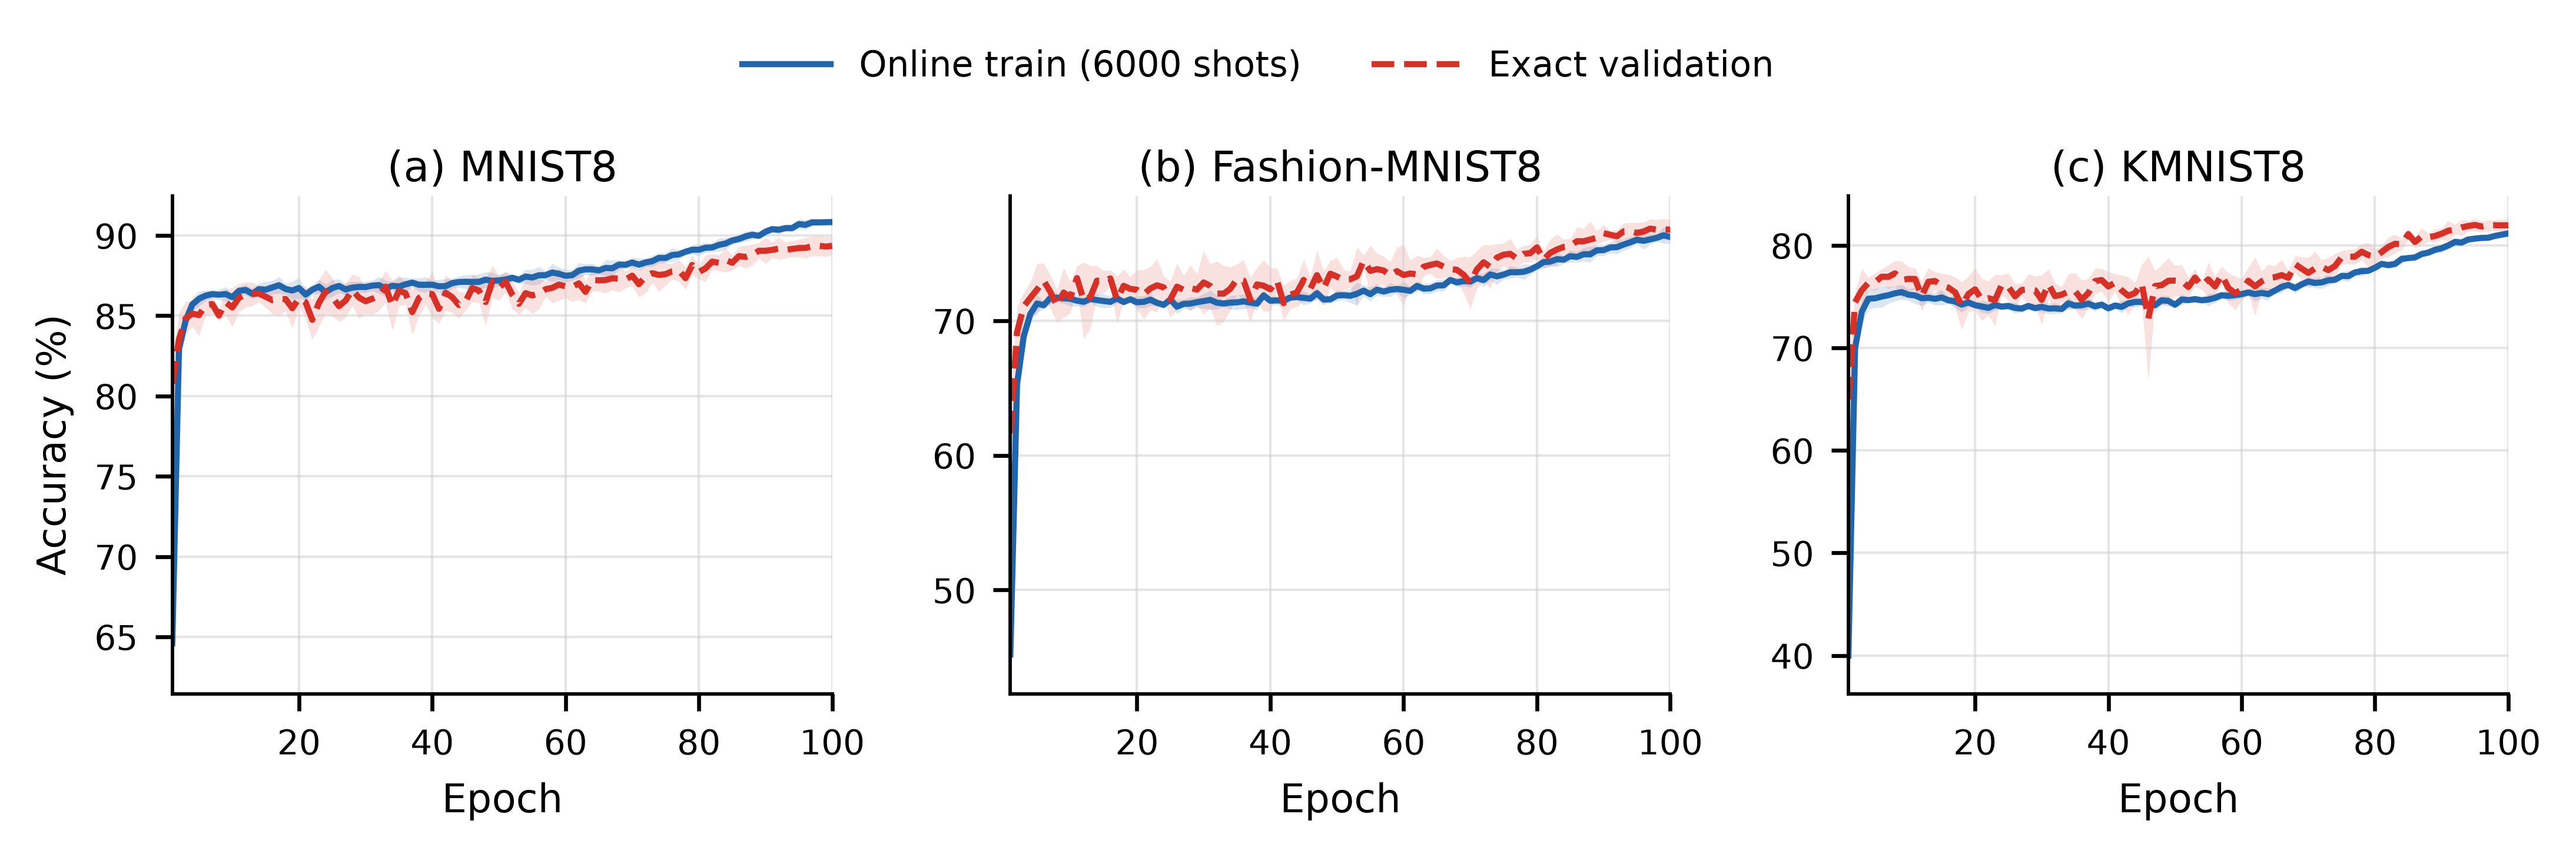
\includegraphics[width=\textwidth]{qfnn_training_trajectories_v6.png}
\caption{Training trajectories for the validation-selected QFNN recipes,
shown as mean $\pm$ sample standard deviation over six independently trained
seeds. Solid blue curves denote online training accuracy obtained with
6000-shot multinomial sampling; dashed red curves denote exact validation
accuracy.}
\label{fig:qfnn-proof-of-concept-curves}
\end{figure}

\clearpage
\twocolumn
\nobalance

\section{Interference-phase modulation}
\label{app:phase}
% ============================================================

A single $R_z(\varphi)$ on the shared interference qubit before the final
Hadamard attaches the same coherent coefficient to every addressed branch
response. Up to a global phase, the branch-one arm acquires
$e^{i\varphi}$, so
\begin{equation}
 \Pr(c=0)
 =\frac{1+\operatorname{Re}[e^{i\varphi}\bra\psi V\ket\psi]}{2}.
\end{equation}
For the unphased reflection sequence,
$\bra\psi V\ket\psi=T_d(2p-1)$ is real, and the centered response becomes
\begin{equation}
 \cos(\varphi)T_d(2p-1).
\end{equation}
This phase modulation provides a simple coherent coefficient for a branch
response. It is particularly useful between deep QFNN layers, where such
coefficients can be introduced without measuring and re-encoding the hidden
state. Independent branch coefficients require the address-controlled
operation
\begin{equation}
 \sum_j\proj{j}_{A}\otimes R_z(\varphi_j),
\end{equation}
which yields $\cos(\varphi_j)T_d(2p_j-1)$ in branch $j$. This modulation
preserves the polynomial degree. The Universal Approximation Theorems use the
more general affine combinations stated in their hypotheses. The numerical
experiment is unphased.

\section{Numerical sanity checks}
\label{app:numerics}

Independent small-dimensional calculations were used as diagnostics, not as
substitutes for the proofs. Random finite-dimensional projectors verified
Theorem~\ref{thm:reflection-chebyshev} to floating-point precision for
multiple ranks and degrees. Sampled coherent projectors achieved ranks
$9$ for $(n,D)=(2,2)$, $16$ for $(2,3)$, and $36$ for $(3,2)$, matching
$\binom{n+D-1}{D}^2$. The interpolation construction reproduced Kronecker
values on random distinct pure states, and exhaustive linear-separator checks
for the equatorial example gave the predicted $D-1$ minimum errors. Random
pure-state Gram matrices also satisfied the nondecreasing effective-dimension
property in Proposition~\ref{prop:effective-dimension-monotone} across the
tested degrees and ridge values. Random finite multiclass banks satisfied the
diagonal-head compilation identity in
Corollary~\ref{cor:deep-diagonal-density} with maximum discrepancy
$7.2\times10^{-15}$. The accompanying sanity-check script reproduces these
diagnostics and is available in the repository cited below; the analytic
theorem statements are established by the proofs in the main text.

% ============================================================
\section*{Declarations}
% ============================================================

\subsection*{Funding}
No funding was received for conducting this study.

\subsection*{Competing interests}
The authors have no relevant financial or non-financial interests to disclose.

\subsection*{Data availability}
No new dataset was created for this study. The numerical experiments use the
publicly available MNIST, Fashion-MNIST, and KMNIST datasets, restricted to
their original labels $0,\ldots,7$.

\subsection*{Code availability}
The QFNN implementation, theorem sanity checks, and complete reproducibility
materials for the numerical experiments are available in the public repository
\url{https://github.com/KiyoLelou10/QFFN}. The archived materials include run configurations, optimization
records, selected recipes, per-seed histories and checkpoints, aggregate
result tables, and plotting data.

\subsection*{Author contributions}
The authors should insert a contribution statement before submission.

% ============================================================
% Self-contained bibliography: no external .bib file is required.
% ============================================================
\begin{thebibliography}{99}

\bibitem[Abbas et~al.(2021)Abbas, Sutter, Zoufal, Lucchi, Figalli, and
Woerner]{abbas2021power}
Abbas A, Sutter D, Zoufal C, Lucchi A, Figalli A, Woerner S (2021) The power
of quantum neural networks. Nat Comput Sci 1:403--409.
\url{https://doi.org/10.1038/s43588-021-00084-1}

\bibitem[Akiba et~al.(2019)Akiba, Sano, Yanase, Ohta, and
Koyama]{akiba2019optuna}
Akiba T, Sano S, Yanase T, Ohta T, Koyama M (2019) Optuna: a next-generation
hyperparameter optimization framework. In: Proceedings of the 25th ACM SIGKDD
International Conference on Knowledge Discovery \& Data Mining, pp 2623--2631.
\url{https://doi.org/10.1145/3292500.3330701}

\bibitem[Bartlett and Mendelson(2002)]{bartlett2002rademacher}
Bartlett PL, Mendelson S (2002) Rademacher and Gaussian complexities: risk
bounds and structural results. J Mach Learn Res 3:463--482.
\url{https://www.jmlr.org/papers/v3/bartlett02a.html}

\bibitem[Bergstra et~al.(2011)Bergstra, Bardenet, Bengio, and
K{\'e}gl]{bergstra2011algorithms}
Bergstra JS, Bardenet R, Bengio Y, K{\'e}gl B (2011) Algorithms for
hyper-parameter optimization. In: Advances in Neural Information Processing
Systems 24.
\url{https://papers.nips.cc/paper/4443}

\bibitem[Beals et~al.(2001)Beals, Buhrman, Cleve, Mosca, and
de~Wolf]{beals2001polynomial}
Beals R, Buhrman H, Cleve R, Mosca M, de~Wolf R (2001) Quantum lower bounds
by polynomials. J ACM 48:778--797.
\url{https://doi.org/10.1145/502090.502097}

\bibitem[Beer et~al.(2020)Beer, Bondarenko, Farrelly, Osborne, Salzmann,
Scheiermann, and Wolf]{beer2020training}
Beer K, Bondarenko D, Farrelly T, Osborne TJ, Salzmann R, Scheiermann D,
Wolf R (2020) Training deep quantum neural networks. Nat Commun 11:808.
\url{https://doi.org/10.1038/s41467-020-14454-2}

\bibitem[Brassard et~al.(2002)Brassard, H{\o}yer, Mosca, and
Tapp]{brassard2002amplitude}
Brassard G, H{\o}yer P, Mosca M, Tapp A (2002) Quantum amplitude amplification
and estimation. In: Lomonaco SJ, Brandt HE (eds) Quantum Computation and
Information. AMS, Providence, pp 53--74.
\url{https://doi.org/10.1090/conm/305/05215}

\bibitem[Cao et~al.(2017)Cao, Guerreschi, and Aspuru-Guzik]{cao2017neuron}
Cao Y, Guerreschi GG, Aspuru-Guzik A (2017) Quantum neuron: an elementary
building block for machine learning on quantum computers.
arXiv:1711.11240. \url{https://arxiv.org/abs/1711.11240}

\bibitem[Caro et~al.(2022)Caro, Huang, Cerezo, Sharma, Sornborger,
Cincio, and Coles]{caro2022generalization}
Caro MC, Huang HY, Cerezo M, et al (2022) Generalization in quantum machine
learning from few training data. Nat Commun 13:4919.
\url{https://doi.org/10.1038/s41467-022-32550-3}

\bibitem[Cerezo et~al.(2021)Cerezo, Sone, Volkoff, Cincio, and
Coles]{cerezo2021cost}
Cerezo M, Sone A, Volkoff T, Cincio L, Coles PJ (2021) Cost function
dependent barren plateaus in shallow parametrized quantum circuits.
Nat Commun 12:1791.
\url{https://doi.org/10.1038/s41467-021-21728-w}

\bibitem[Chiribella et~al.(2009)Chiribella, D'Ariano, and
Perinotti]{chiribella2009networks}
Chiribella G, D'Ariano GM, Perinotti P (2009) Theoretical framework for
quantum networks. Phys Rev A 80:022339.
\url{https://doi.org/10.1103/PhysRevA.80.022339}

\bibitem[Clanuwat et~al.(2018)Clanuwat, Bober-Irizar, Kitamoto, Lamb,
Yamamoto, and Ha]{clanuwat2018deep}
Clanuwat T, Bober-Irizar M, Kitamoto A, Lamb A, Yamamoto K, Ha D (2018) Deep
learning for classical Japanese literature. arXiv:1812.01718.
\url{https://arxiv.org/abs/1812.01718}

\bibitem[Cybenko(1989)]{cybenko1989approximation}
Cybenko G (1989) Approximation by superpositions of a sigmoidal function.
Math Control Signals Syst 2:303--314.
\url{https://doi.org/10.1007/BF02551274}

\bibitem[Daniely(2017)]{daniely2017depth}
Daniely A (2017) Depth separation for neural networks. In: Proceedings of
the 30th Conference on Learning Theory, PMLR 65:690--696.
\url{https://proceedings.mlr.press/v65/daniely17a.html}

\bibitem[Eldan and Shamir(2016)]{eldan2016power}
Eldan R, Shamir O (2016) The power of depth for feedforward neural networks.
In: Proceedings of the 29th Annual Conference on Learning Theory, PMLR
49:907--940. \url{https://proceedings.mlr.press/v49/eldan16.html}

\bibitem[Gil-Fuster et~al.(2024)Gil-Fuster, Eisert, and
Bravo-Prieto]{gilfuster2024rethinking}
Gil-Fuster E, Eisert J, Bravo-Prieto C (2024) Understanding quantum machine
learning also requires rethinking generalization.
Nat Commun 15:2277.
\url{https://doi.org/10.1038/s41467-024-45882-z}

\bibitem[Gily{\'e}n et~al.(2019)Gily{\'e}n, Su, Low, and
Wiebe]{gilyen2019qsvt}
Gily{\'e}n A, Su Y, Low GH, Wiebe N (2019) Quantum singular value
transformation and beyond: exponential improvements for quantum matrix
arithmetics. In: Proceedings of the 51st Annual ACM SIGACT Symposium on
Theory of Computing, pp 193--204.
\url{https://doi.org/10.1145/3313276.3316366}

\bibitem[Hur and Park(2025)]{hur2025margins}
Hur T, Park DK (2025) Understanding generalization in quantum machine
learning with margins. In: Proceedings of the 42nd International Conference
on Machine Learning, PMLR 267:26338--26360.
\url{https://proceedings.mlr.press/v267/hur25a.html}

\bibitem[Iten et~al.(2016)Iten, Colbeck, Kukuljan, Home, and
Christandl]{iten2016isometries}
Iten R, Colbeck R, Kukuljan I, Home J, Christandl M (2016) Quantum circuits
for isometries. Phys Rev A 93:032318.
\url{https://doi.org/10.1103/PhysRevA.93.032318}

\bibitem[Ivashkov et~al.(2026)Ivashkov, Huang, Koor, Pira, and
Rebentrost]{ivashkov2026qkan}
Ivashkov P, Huang PW, Koor K, Pira L, Rebentrost P (2026) QKAN: quantum
Kolmogorov--Arnold networks with applications in machine learning and
multivariate state preparation. npj Quantum Inf 12:73.
\url{https://doi.org/10.1038/s41534-026-01202-5}

\bibitem[Jerbi et~al.(2023)Jerbi, Fiderer, Poulsen Nautrup, K{\"u}bler,
Briegel, and Dunjko]{jerbi2023beyond}
Jerbi S, Fiderer LJ, Poulsen Nautrup H, K{\"u}bler JM, Briegel HJ, Dunjko V
(2023) Quantum machine learning beyond kernel methods. Nat Commun 14:517.
\url{https://doi.org/10.1038/s41467-023-36159-y}

\bibitem[LeCun et~al.(1998)LeCun, Bottou, Bengio, and
Haffner]{lecun1998gradient}
LeCun Y, Bottou L, Bengio Y, Haffner P (1998) Gradient-based learning applied
to document recognition. Proc IEEE 86(11):2278--2324.
\url{https://doi.org/10.1109/5.726791}

\bibitem[Li et~al.(2024)Li, Salek, Wang, and Chowdhury]{li2024qcpn}
Li S, Salek MS, Wang Y, Chowdhury M (2024) Quantum-inspired activation
functions and quantum Chebyshev-polynomial network. arXiv:2404.05901.
\url{https://arxiv.org/abs/2404.05901}

\bibitem[Low and Chuang(2017)]{low2017qsp}
Low GH, Chuang IL (2017) Optimal Hamiltonian simulation by quantum signal
processing. Phys Rev Lett 118:010501.
\url{https://doi.org/10.1103/PhysRevLett.118.010501}

\bibitem[Maronese et~al.(2022)Maronese, Destri, and
Prati]{maronese2022activation}
Maronese M, Destri C, Prati E (2022) Quantum activation functions for
quantum neural networks. Quantum Inf Process 21:128.
\url{https://doi.org/10.1007/s11128-022-03466-0}

\bibitem[McClean et~al.(2018)McClean, Boixo, Smelyanskiy, Babbush, and
Neven]{mcclean2018barren}
McClean JR, Boixo S, Smelyanskiy VN, Babbush R, Neven H (2018) Barren
plateaus in quantum neural network training landscapes. Nat Commun 9:4812.
\url{https://doi.org/10.1038/s41467-018-07090-4}

\bibitem[Mele et~al.(2026)Mele, Angrisani, Ghosh, Khatri, Eisert,
Stilck Fran{\c c}a, and Quek]{mele2026noise}
Mele AA, Angrisani A, Ghosh S, Khatri S, Eisert J, Stilck Fran{\c c}a D,
Quek Y (2026) Noise-induced shallow circuits and the absence of barren
plateaus. Nat Phys 22:751--756.
\url{https://doi.org/10.1038/s41567-026-03245-z}

\bibitem[Mhaskar and Poggio(2016)]{mhaskar2016deep}
Mhaskar H, Poggio T (2016) Deep vs. shallow networks: an approximation
theory perspective. Anal Appl 14:829--848.
\url{https://doi.org/10.1142/S0219530516400042}

\bibitem[P{\'e}rez-Salinas et~al.(2020)P{\'e}rez-Salinas,
Cervera-Lierta, Gil-Fuster, and Latorre]{perezsalinas2020reuploading}
P{\'e}rez-Salinas A, Cervera-Lierta A, Gil-Fuster E, Latorre JI (2020)
Data re-uploading for a universal quantum classifier. Quantum 4:226.
\url{https://doi.org/10.22331/q-2020-02-06-226}

\bibitem[Schuld and Killoran(2019)]{schuld2019feature}
Schuld M, Killoran N (2019) Quantum machine learning in feature Hilbert
spaces. Phys Rev Lett 122:040504.
\url{https://doi.org/10.1103/PhysRevLett.122.040504}

\bibitem[Schuld(2021)]{schuld2021kernel}
Schuld M (2021) Supervised quantum machine learning models are kernel
methods. arXiv:2101.11020. \url{https://arxiv.org/abs/2101.11020}

\bibitem[Schuld et~al.(2021)Schuld, Sweke, and Meyer]{schuld2021encoding}
Schuld M, Sweke R, Meyer JJ (2021) Effect of data encoding on the expressive
power of variational quantum-machine-learning models. Phys Rev A 103:032430.
\url{https://doi.org/10.1103/PhysRevA.103.032430}

\bibitem[Singh et~al.(2024)Singh, Goldberg, and Heshami]{singh2024coherent}
Singh U, Goldberg AZ, Heshami K (2024) Coherent feed-forward quantum neural
network. Quantum Mach Intell 6:89.
\url{https://doi.org/10.1007/s42484-024-00222-8}

\bibitem[Stone(1948)]{stone1948weierstrass}
Stone MH (1948) The generalized Weierstrass approximation theorem.
Math Mag 21:167--184.
\url{https://doi.org/10.2307/3029750}

\bibitem[Tacchino et~al.(2020)Tacchino, Barkoutsos, Macchiavello,
Tavernelli, Gerace, and Bajoni]{tacchino2020feedforward}
Tacchino F, Barkoutsos P, Macchiavello C, Tavernelli I, Gerace D, Bajoni D
(2020) Quantum implementation of an artificial feed-forward neural network.
Quantum Sci Technol 5:044010.
\url{https://doi.org/10.1088/2058-9565/abb8e4}

\bibitem[Telgarsky(2016)]{telgarsky2016benefits}
Telgarsky M (2016) Benefits of depth in neural networks. In: Proceedings of
the 29th Annual Conference on Learning Theory, PMLR 49:1517--1539.
\url{https://proceedings.mlr.press/v49/telgarsky16.html}

\bibitem[Trefethen(2019)]{trefethen2019approximation}
Trefethen LN (2019) Approximation Theory and Approximation Practice,
extended edn. Society for Industrial and Applied Mathematics, Philadelphia.
\url{https://doi.org/10.1137/1.9781611975949}

\bibitem[Wang et~al.(2021)Wang, Fontana, Cerezo, Sharma, Sone,
Cincio, and Coles]{wang2021noise}
Wang S, Fontana E, Cerezo M, et al (2021) Noise-induced barren plateaus in
variational quantum algorithms. Nat Commun 12:6961.
\url{https://doi.org/10.1038/s41467-021-27045-6}

\bibitem[Xiao et~al.(2017)Xiao, Rasul, and Vollgraf]{xiao2017fashion}
Xiao H, Rasul K, Vollgraf R (2017) Fashion-MNIST: a novel image dataset for
benchmarking machine learning algorithms. arXiv:1708.07747.
\url{https://arxiv.org/abs/1708.07747}

\end{thebibliography}

\end{document}
